\documentclass{article}\usepackage[]{graphicx}\usepackage[]{color}
%% maxwidth is the original width if it is less than linewidth
%% otherwise use linewidth (to make sure the graphics do not exceed the margin)
\makeatletter
\def\maxwidth{ %
  \ifdim\Gin@nat@width>\linewidth
    \linewidth
  \else
    \Gin@nat@width
  \fi
}
\makeatother

\definecolor{fgcolor}{rgb}{0.345, 0.345, 0.345}
\newcommand{\hlnum}[1]{\textcolor[rgb]{0.686,0.059,0.569}{#1}}%
\newcommand{\hlstr}[1]{\textcolor[rgb]{0.192,0.494,0.8}{#1}}%
\newcommand{\hlcom}[1]{\textcolor[rgb]{0.678,0.584,0.686}{\textit{#1}}}%
\newcommand{\hlopt}[1]{\textcolor[rgb]{0,0,0}{#1}}%
\newcommand{\hlstd}[1]{\textcolor[rgb]{0.345,0.345,0.345}{#1}}%
\newcommand{\hlkwa}[1]{\textcolor[rgb]{0.161,0.373,0.58}{\textbf{#1}}}%
\newcommand{\hlkwb}[1]{\textcolor[rgb]{0.69,0.353,0.396}{#1}}%
\newcommand{\hlkwc}[1]{\textcolor[rgb]{0.333,0.667,0.333}{#1}}%
\newcommand{\hlkwd}[1]{\textcolor[rgb]{0.737,0.353,0.396}{\textbf{#1}}}%

\usepackage{framed}
\makeatletter
\newenvironment{kframe}{%
 \def\at@end@of@kframe{}%
 \ifinner\ifhmode%
  \def\at@end@of@kframe{\end{minipage}}%
  \begin{minipage}{\columnwidth}%
 \fi\fi%
 \def\FrameCommand##1{\hskip\@totalleftmargin \hskip-\fboxsep
 \colorbox{shadecolor}{##1}\hskip-\fboxsep
     % There is no \\@totalrightmargin, so:
     \hskip-\linewidth \hskip-\@totalleftmargin \hskip\columnwidth}%
 \MakeFramed {\advance\hsize-\width
   \@totalleftmargin\z@ \linewidth\hsize
   \@setminipage}}%
 {\par\unskip\endMakeFramed%
 \at@end@of@kframe}
\makeatother

\definecolor{shadecolor}{rgb}{.97, .97, .97}
\definecolor{messagecolor}{rgb}{0, 0, 0}
\definecolor{warningcolor}{rgb}{1, 0, 1}
\definecolor{errorcolor}{rgb}{1, 0, 0}
\newenvironment{knitrout}{}{} % an empty environment to be redefined in TeX

\usepackage{alltt}

\usepackage[margin = 1in]{geometry}
\usepackage{float, enumitem}
\usepackage{graphicx}
\usepackage{amsmath}

\setlength{\topsep}{0pt}
\setlength{\parskip}{0pt}
\setlength{\partopsep}{1pt}

\renewcommand\thesubsection{\thesection (\alph{subsection})}
\IfFileExists{upquote.sty}{\usepackage{upquote}}{}
\begin{document}

\title{ASSIGNMENT 3}
\author{Brandon Lampe \\ STAT 527 \\ Advanced Data Analysis I}
\maketitle

\section{Cloud seeding:}
\subsection{(10 pts) Carefully check the assumption of normality of the data on the original scale by describing the shape of the data distribution and the sampling distribution of the mean (using the bootstrap). You need to do the seeded and unseeded days separately.}

\begin{knitrout}
\definecolor{shadecolor}{rgb}{0.969, 0.969, 0.969}\color{fgcolor}\begin{kframe}
\begin{alltt}
\hlcom{# Load libraries and source functions for analysis}
\hlkwd{library}\hlstd{(ggplot2)}
\hlkwd{library}\hlstd{(grid)}
\hlkwd{library}\hlstd{(gridExtra)}
\hlkwd{library}\hlstd{(reshape2)}
\hlkwd{library}\hlstd{(car)}
\hlkwd{source}\hlstd{(}\hlstr{"ADA1_FUNC.R"}\hlstd{)}

\hlcom{# read in cloud seeding data}
\hlstd{d1.initial} \hlkwb{<-} \hlkwd{read.csv}\hlstd{(}\hlstr{"http://statacumen.com/teach/ADA1/ADA1_HW_02_F14-1.csv"}\hlstd{)}
\hlstd{LogS} \hlkwb{<-} \hlkwd{log}\hlstd{(d1.initial}\hlopt{$}\hlstd{seeded)}             \hlcom{# log of seeded data}
\hlstd{LogUS} \hlkwb{<-} \hlkwd{log}\hlstd{(d1.initial}\hlopt{$}\hlstd{unseeded)}          \hlcom{# log of unseeded data}
\hlstd{d1} \hlkwb{<-} \hlkwd{data.frame}\hlstd{(}\hlkwd{cbind}\hlstd{(d1.initial,LogUS, LogS ))}   \hlcom{# all data}
\end{alltt}
\end{kframe}
\end{knitrout}

%%%%%%%%%%%%%%%%%%%%%%%%%%
%% PROB 1 A
%%%%%%%%%%%%%%%%%%%%%%%%%%


\begin{knitrout}
\definecolor{shadecolor}{rgb}{0.969, 0.969, 0.969}\color{fgcolor}\begin{kframe}
\begin{alltt}
\hlcom{# histogram of Unseeded Precip}
\hlstd{Precip.hist} \hlkwb{<-} \hlkwd{ggplot}\hlstd{(d1,} \hlkwd{aes}\hlstd{(}\hlkwc{x} \hlstd{= unseeded))}
\hlstd{Precip.hist} \hlkwb{<-} \hlstd{Precip.hist} \hlopt{+} \hlkwd{geom_histogram}\hlstd{(}\hlkwc{binwidth} \hlstd{=} \hlnum{100}\hlstd{,}\hlkwc{color} \hlstd{=} \hlstr{"black"}\hlstd{,}
                                            \hlkwc{fill} \hlstd{=} \hlstr{"white"}\hlstd{)}
\hlstd{Precip.hist} \hlkwb{<-} \hlstd{Precip.hist} \hlopt{+} \hlkwd{labs}\hlstd{(}\hlkwc{title} \hlstd{=} \hlstr{"Precipitation, Unseeded"}\hlstd{)}

\hlcom{# boxplot of Unseeded Precip}
\hlstd{Precip.box} \hlkwb{<-} \hlkwd{ggplot}\hlstd{(d1,} \hlkwd{aes}\hlstd{(}\hlkwc{x} \hlstd{=} \hlstr{"Precipitation"}\hlstd{,}\hlkwc{y} \hlstd{= unseeded))} \hlcom{# boxplot of Precip}
\hlstd{Precip.box} \hlkwb{<-} \hlstd{Precip.box} \hlopt{+} \hlkwd{geom_boxplot}\hlstd{()}
\hlstd{Precip.box} \hlkwb{<-} \hlstd{Precip.box} \hlopt{+} \hlkwd{coord_flip}\hlstd{()}
\hlstd{Precip.box} \hlkwb{<-} \hlstd{Precip.box} \hlopt{+} \hlkwd{stat_summary}\hlstd{(}\hlkwc{fun.y} \hlstd{= mean,} \hlkwc{geom} \hlstd{=} \hlstr{"point"}\hlstd{,}
                                        \hlkwc{shape} \hlstd{=} \hlnum{3}\hlstd{,} \hlkwc{size} \hlstd{=} \hlnum{4}\hlstd{)}
\end{alltt}
\end{kframe}
\end{knitrout}

\begin{figure}[H]  \begin{center}
\begin{knitrout}
\definecolor{shadecolor}{rgb}{0.969, 0.969, 0.969}\color{fgcolor}\begin{kframe}
\begin{alltt}
\hlcom{# plot histogram and boxplot}
\hlkwd{grid.arrange}\hlstd{(Precip.hist, Precip.box,} \hlkwc{nrow} \hlstd{=} \hlnum{2}\hlstd{)}
\end{alltt}
\end{kframe}
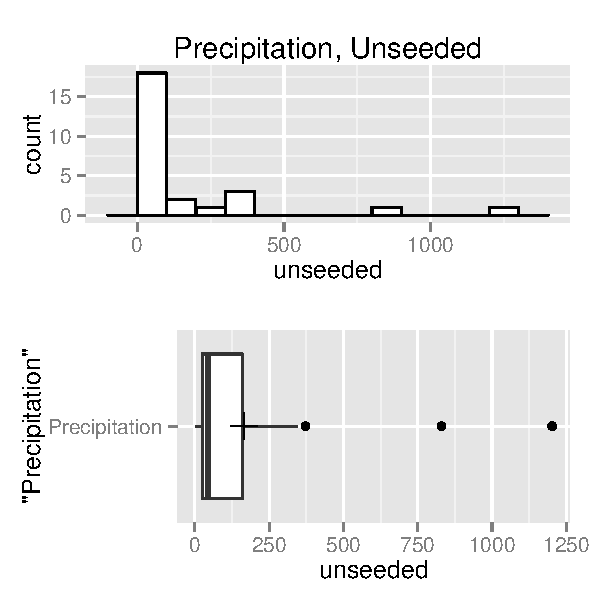
\includegraphics[width=\maxwidth]{figure/1a_data_unseed_plot} 

\end{knitrout}
\end{center} \caption{Histogram and Boxplot of Unseeded Data Distribution.} \end{figure}


\begin{figure}[H]  \begin{center} \vspace{-0.45in}
\begin{knitrout}
\definecolor{shadecolor}{rgb}{0.969, 0.969, 0.969}\color{fgcolor}\begin{kframe}
\begin{alltt}
\hlcom{# qq plot for unseeded data}
\hlkwd{qqPlot}\hlstd{(d1}\hlopt{$}\hlstd{unseeded,} \hlkwc{las} \hlstd{=} \hlnum{1}\hlstd{,} \hlkwc{id.n} \hlstd{=} \hlnum{0}\hlstd{,} \hlkwc{id.cex} \hlstd{=} \hlnum{1}\hlstd{,} \hlkwc{lwd} \hlstd{=} \hlnum{1}\hlstd{,} \hlkwc{ylab} \hlstd{=} \hlstr{"Precipitation"}\hlstd{)}
\end{alltt}
\end{kframe}
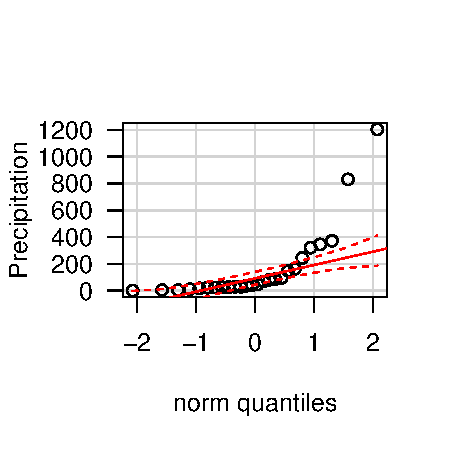
\includegraphics[width=\maxwidth]{figure/1a_qq_unseed} 

\end{knitrout}
\end{center}\caption{QQ Plot of Unseeded Data Distribution.} \end{figure}


\begin{itemize}
\item Unseeded Data Distribtion:  The unseeded data distribution is unimodal, skewed right, and contains outliers.  The mean of the data is outside of the IQR.  This shape occurs because only positive valued data are possible. The QQ plot of the data shows  the data are not normally distributed, as they deviate substantially from the line representing normality and more than 5\% of the data are outside of the limits.
\end{itemize}

\vspace{-0.45in}

\begin{figure}[H]  \begin{center}
\begin{knitrout}
\definecolor{shadecolor}{rgb}{0.969, 0.969, 0.969}\color{fgcolor}\begin{kframe}
\begin{alltt}
\hlstd{unseed.samp} \hlkwb{<-} \hlkwd{bs.one.samp.dist}\hlstd{(d1}\hlopt{$}\hlstd{unseeded)}  \hlcom{# bootstrap of unseeded data}
\end{alltt}
\end{kframe}
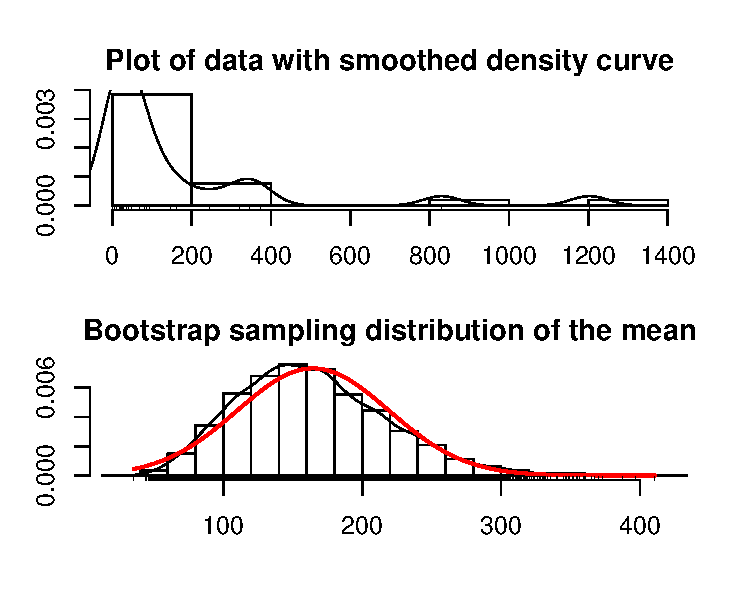
\includegraphics[width=\maxwidth]{figure/1a_boot_unseed} 
\begin{kframe}\begin{alltt}
\hlstd{unseed.samp.df} \hlkwb{<-} \hlkwd{data.frame}\hlstd{(unseed.samp)}
\end{alltt}
\end{kframe}
\end{knitrout}
\end{center} \caption{Resuts of Sampling Distribution from Bootstrap Function of Unseeded Data.} \end{figure}


\begin{knitrout}
\definecolor{shadecolor}{rgb}{0.969, 0.969, 0.969}\color{fgcolor}\begin{kframe}
\begin{alltt}
\hlcom{# histogram of Unseeded Precip}
\hlstd{Samp.hist} \hlkwb{<-} \hlkwd{ggplot}\hlstd{(unseed.samp.df,} \hlkwd{aes}\hlstd{(}\hlkwc{x} \hlstd{= unseed.samp))}
\hlstd{Samp.hist} \hlkwb{<-} \hlstd{Samp.hist} \hlopt{+} \hlkwd{geom_histogram}\hlstd{(}\hlkwc{binwidth} \hlstd{=} \hlnum{10}\hlstd{,}\hlkwc{color} \hlstd{=} \hlstr{"black"}\hlstd{,}
                                            \hlkwc{fill} \hlstd{=} \hlstr{"white"}\hlstd{)}
\hlstd{Samp.hist} \hlkwb{<-} \hlstd{Samp.hist} \hlopt{+} \hlkwd{labs}\hlstd{(}\hlkwc{title} \hlstd{=} \hlstr{"Precipitation, Bootstrap Sample of Unseeded"}\hlstd{)}

\hlcom{# boxplot of Unseeded Precip}
\hlstd{Samp.box} \hlkwb{<-} \hlkwd{ggplot}\hlstd{(unseed.samp.df,} \hlkwd{aes}\hlstd{(}\hlkwc{x} \hlstd{=} \hlstr{"Precipitation"}\hlstd{,}\hlkwc{y} \hlstd{= unseed.samp))} \hlcom{# boxplot of Precip}
\hlstd{Samp.box} \hlkwb{<-} \hlstd{Samp.box} \hlopt{+} \hlkwd{geom_boxplot}\hlstd{()}
\hlstd{Samp.box} \hlkwb{<-} \hlstd{Samp.box} \hlopt{+} \hlkwd{coord_flip}\hlstd{()}
\hlstd{Samp.box} \hlkwb{<-} \hlstd{Samp.box} \hlopt{+} \hlkwd{stat_summary}\hlstd{(}\hlkwc{fun.y} \hlstd{= mean,} \hlkwc{geom} \hlstd{=} \hlstr{"point"}\hlstd{,}
                                        \hlkwc{shape} \hlstd{=} \hlnum{3}\hlstd{,} \hlkwc{size} \hlstd{=} \hlnum{4}\hlstd{)}
\end{alltt}
\end{kframe}
\end{knitrout}

\begin{figure}[H]  \begin{center} \vspace{-0.45in}
\begin{knitrout}
\definecolor{shadecolor}{rgb}{0.969, 0.969, 0.969}\color{fgcolor}\begin{kframe}
\begin{alltt}
\hlcom{# plot histogram and boxplot}
\hlkwd{grid.arrange}\hlstd{(Samp.hist, Samp.box,} \hlkwc{nrow} \hlstd{=} \hlnum{2}\hlstd{)}
\end{alltt}
\end{kframe}
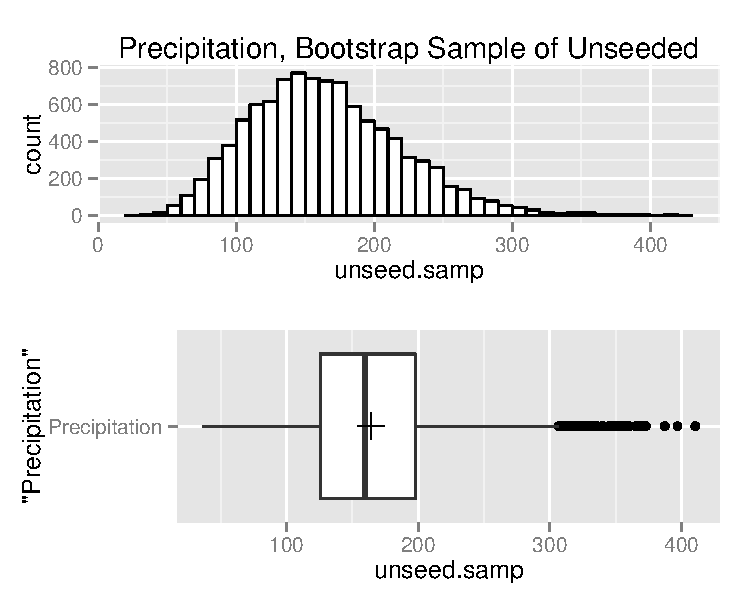
\includegraphics[width=\maxwidth]{figure/1a_box_unseed_plot} 

\end{knitrout}
\end{center}\caption{Histogram and Boxplot of Bootstrap Sample Distribution of Unseeded Data.} \end{figure}

\begin{figure}[H]  \begin{center}
\begin{knitrout}
\definecolor{shadecolor}{rgb}{0.969, 0.969, 0.969}\color{fgcolor}\begin{kframe}
\begin{alltt}
\hlcom{# qq plot for bootstrap sampling distribution of unseeded data}
\hlkwd{qqPlot}\hlstd{(unseed.samp,} \hlkwc{las} \hlstd{=} \hlnum{1}\hlstd{,} \hlkwc{id.n} \hlstd{=} \hlnum{0}\hlstd{,} \hlkwc{id.cex} \hlstd{=} \hlnum{1}\hlstd{,} \hlkwc{lwd} \hlstd{=} \hlnum{1}\hlstd{,} \hlkwc{ylab} \hlstd{=} \hlstr{"Precipitation"}\hlstd{)}
\end{alltt}
\end{kframe}
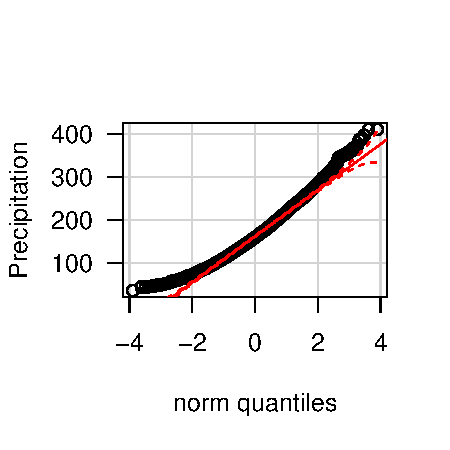
\includegraphics[width=\maxwidth]{figure/1a_qq_unseedsamp} 

\end{knitrout}
\end{center} \caption{QQ Plot of Bootstrap Sampling Distribution of Unseeded Data.} \end{figure}

\begin{itemize}
\item Unseeded Bootsrap Sample Distribtion:  The sampled distribution is unimodal, skewed right, and contains outliers.  The mean of the data is near the mean.  The QQ plot of the sample data shows they are not normally distributed; as they deviate substantially from the line representing normality and far more than 5\% of the data are outside of the limits.
\end{itemize}

%% ==========================================
%% seeded data
%% ==========================================

\begin{knitrout}
\definecolor{shadecolor}{rgb}{0.969, 0.969, 0.969}\color{fgcolor}\begin{kframe}
\begin{alltt}
\hlcom{# histogram of Seeded Precip}
\hlstd{Precip.hist.seed} \hlkwb{<-} \hlkwd{ggplot}\hlstd{(d1,} \hlkwd{aes}\hlstd{(}\hlkwc{x} \hlstd{= seeded))}
\hlstd{Precip.hist.seed} \hlkwb{<-} \hlstd{Precip.hist.seed} \hlopt{+} \hlkwd{geom_histogram}\hlstd{(}\hlkwc{binwidth} \hlstd{=} \hlnum{100}\hlstd{,}\hlkwc{color} \hlstd{=} \hlstr{"black"}\hlstd{,}
                                            \hlkwc{fill} \hlstd{=} \hlstr{"white"}\hlstd{)}
\hlstd{Precip.hist.seed} \hlkwb{<-} \hlstd{Precip.hist.seed} \hlopt{+} \hlkwd{labs}\hlstd{(}\hlkwc{title} \hlstd{=} \hlstr{"Precipitation, Seeded"}\hlstd{)}

\hlcom{# boxplot of Seeded Precip}
\hlstd{Precip.box.seed} \hlkwb{<-} \hlkwd{ggplot}\hlstd{(d1,} \hlkwd{aes}\hlstd{(}\hlkwc{x} \hlstd{=} \hlstr{"Precipitation"}\hlstd{,}\hlkwc{y} \hlstd{= seeded))} \hlcom{# boxplot of Precip}
\hlstd{Precip.box.seed} \hlkwb{<-} \hlstd{Precip.box.seed} \hlopt{+} \hlkwd{geom_boxplot}\hlstd{()}
\hlstd{Precip.box.seed} \hlkwb{<-} \hlstd{Precip.box.seed} \hlopt{+} \hlkwd{coord_flip}\hlstd{()}
\hlstd{Precip.box.seed} \hlkwb{<-} \hlstd{Precip.box.seed} \hlopt{+} \hlkwd{stat_summary}\hlstd{(}\hlkwc{fun.y} \hlstd{= mean,} \hlkwc{geom} \hlstd{=} \hlstr{"point"}\hlstd{,}
                                        \hlkwc{shape} \hlstd{=} \hlnum{3}\hlstd{,} \hlkwc{size} \hlstd{=} \hlnum{4}\hlstd{)}
\end{alltt}
\end{kframe}
\end{knitrout}

\begin{figure}[H]  \begin{center}
\begin{knitrout}
\definecolor{shadecolor}{rgb}{0.969, 0.969, 0.969}\color{fgcolor}\begin{kframe}
\begin{alltt}
\hlcom{# plot histogram and boxplot}
\hlkwd{grid.arrange}\hlstd{(Precip.hist.seed, Precip.box.seed,} \hlkwc{nrow} \hlstd{=} \hlnum{2}\hlstd{)}
\end{alltt}
\end{kframe}
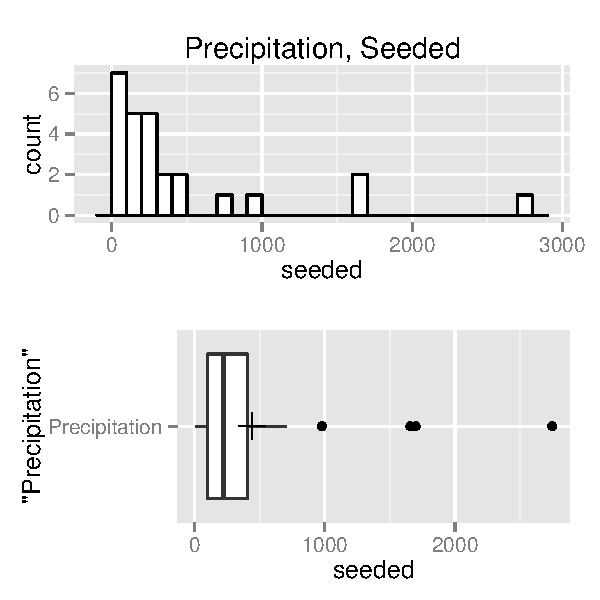
\includegraphics[width=\maxwidth]{figure/1a_data_seed_plot} 

\end{knitrout}
\end{center} \caption{Histogram and Boxplot of Seeded Data Distribution.} \end{figure}


\begin{figure}[H]  \begin{center} \vspace{-0.45in}
\begin{knitrout}
\definecolor{shadecolor}{rgb}{0.969, 0.969, 0.969}\color{fgcolor}\begin{kframe}
\begin{alltt}
\hlcom{# qq plot for Seeded data}
\hlcom{# las = 1 : turns labels on y-axis to read horizontally}
\hlcom{# id.n = n : labels n most extreme observations, and outputs to console}
\hlcom{# id.cex = 1 : is the size of those labels}
\hlcom{# lwd    =  1 : line width}
\hlkwd{qqPlot}\hlstd{(d1}\hlopt{$}\hlstd{seeded,} \hlkwc{las} \hlstd{=} \hlnum{1}\hlstd{,} \hlkwc{id.n} \hlstd{=} \hlnum{0}\hlstd{,} \hlkwc{id.cex} \hlstd{=} \hlnum{1}\hlstd{,} \hlkwc{lwd} \hlstd{=} \hlnum{1}\hlstd{,} \hlkwc{ylab} \hlstd{=} \hlstr{"Precipitation"}\hlstd{)}
\end{alltt}
\end{kframe}
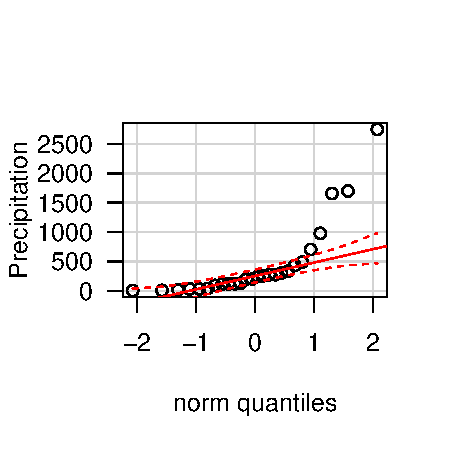
\includegraphics[width=\maxwidth]{figure/1a_qq_seed} 

\end{knitrout}
\end{center}\caption{QQ Plot of Seeded Data Distribution.} \end{figure}


\begin{itemize}
\item Seeded Data Distribtion:  The seeded data distribution is unimodal, skewed right, and contains outliers.  The mean of the data is outside of the IQR.  This shape occurs because only positive valued data are possible. The QQ plot of the data shows  the data are not normally distributed, as they deviate substantially from the line representing normality and more than 5\% of the data are outisde the limits.
\end{itemize}

\vspace{-0.45in}

\begin{figure}[H]  \begin{center}
\begin{knitrout}
\definecolor{shadecolor}{rgb}{0.969, 0.969, 0.969}\color{fgcolor}\begin{kframe}
\begin{alltt}
\hlstd{seed.samp} \hlkwb{<-} \hlkwd{bs.one.samp.dist}\hlstd{(d1}\hlopt{$}\hlstd{seeded)}  \hlcom{# bootstrap of seeded data}
\end{alltt}
\end{kframe}
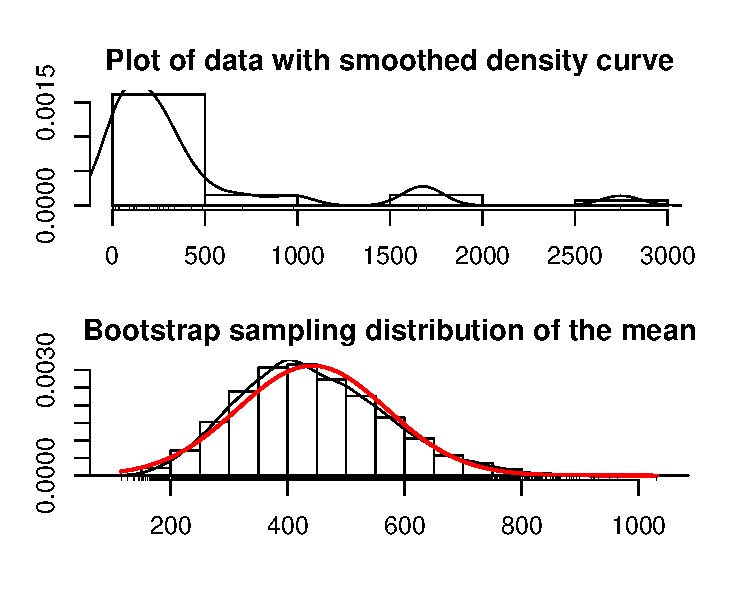
\includegraphics[width=\maxwidth]{figure/1a_boot_seed} 
\begin{kframe}\begin{alltt}
\hlstd{seed.samp.df} \hlkwb{<-} \hlkwd{data.frame}\hlstd{(seed.samp)}
\end{alltt}
\end{kframe}
\end{knitrout}
\end{center} \caption{Resuts of Sampling Distribution from Bootstrap Function of Seeded Data.}
\end{figure}

\begin{knitrout}
\definecolor{shadecolor}{rgb}{0.969, 0.969, 0.969}\color{fgcolor}\begin{kframe}
\begin{alltt}
\hlcom{# histogram of Unseeded Precip}
\hlstd{Samp.hist.seed} \hlkwb{<-} \hlkwd{ggplot}\hlstd{(seed.samp.df,} \hlkwd{aes}\hlstd{(}\hlkwc{x} \hlstd{= seed.samp))}
\hlstd{Samp.hist.seed} \hlkwb{<-} \hlstd{Samp.hist.seed} \hlopt{+} \hlkwd{geom_histogram}\hlstd{(}\hlkwc{binwidth} \hlstd{=} \hlnum{100}\hlstd{,}\hlkwc{color} \hlstd{=} \hlstr{"black"}\hlstd{,}
                                            \hlkwc{fill} \hlstd{=} \hlstr{"white"}\hlstd{)}
\hlstd{Samp.hist.seed} \hlkwb{<-} \hlstd{Samp.hist.seed} \hlopt{+} \hlkwd{labs}\hlstd{(}\hlkwc{title} \hlstd{=} \hlstr{"Precipitation, Bootstrap Sample of Seeded"}\hlstd{)}

\hlcom{# boxplot of Seeded Precip}
\hlstd{Samp.box.seed} \hlkwb{<-} \hlkwd{ggplot}\hlstd{(seed.samp.df,} \hlkwd{aes}\hlstd{(}\hlkwc{x} \hlstd{=} \hlstr{"Precipitation"}\hlstd{,}\hlkwc{y} \hlstd{= seed.samp))} \hlcom{# boxplot of Precip}
\hlstd{Samp.box.seed} \hlkwb{<-} \hlstd{Samp.box.seed} \hlopt{+} \hlkwd{geom_boxplot}\hlstd{()}
\hlstd{Samp.box.seed} \hlkwb{<-} \hlstd{Samp.box.seed} \hlopt{+} \hlkwd{coord_flip}\hlstd{()}
\hlstd{Samp.box.seed} \hlkwb{<-} \hlstd{Samp.box.seed} \hlopt{+} \hlkwd{stat_summary}\hlstd{(}\hlkwc{fun.y} \hlstd{= mean,} \hlkwc{geom} \hlstd{=} \hlstr{"point"}\hlstd{,}
                                        \hlkwc{shape} \hlstd{=} \hlnum{3}\hlstd{,} \hlkwc{size} \hlstd{=} \hlnum{4}\hlstd{)}
\end{alltt}
\end{kframe}
\end{knitrout}

\begin{figure}[H]  \begin{center} \vspace{-0.45in}
\begin{knitrout}
\definecolor{shadecolor}{rgb}{0.969, 0.969, 0.969}\color{fgcolor}\begin{kframe}
\begin{alltt}
\hlcom{# plot histogram and boxplot}
\hlkwd{grid.arrange}\hlstd{(Samp.hist.seed, Samp.box.seed,} \hlkwc{nrow} \hlstd{=} \hlnum{2}\hlstd{)}
\end{alltt}
\end{kframe}
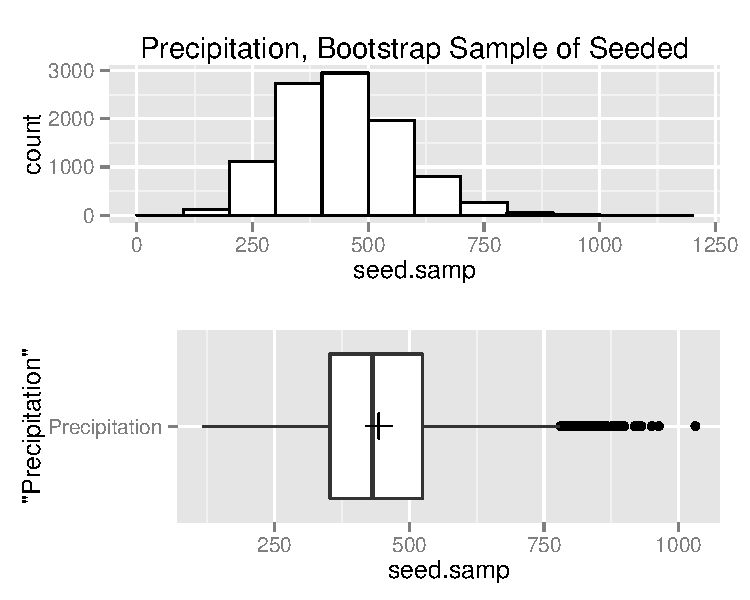
\includegraphics[width=\maxwidth]{figure/1a_box_seed_plot} 

\end{knitrout}
\end{center}\caption{Histogram and Boxplot of Bootstrap Sample Distribution of Seeded Data.} \end{figure}

\begin{figure}[H]  \begin{center}
\begin{knitrout}
\definecolor{shadecolor}{rgb}{0.969, 0.969, 0.969}\color{fgcolor}\begin{kframe}
\begin{alltt}
\hlcom{# qq plot for bootstrap sampling distribution of seeded data}
\hlkwd{qqPlot}\hlstd{(seed.samp,} \hlkwc{las} \hlstd{=} \hlnum{1}\hlstd{,} \hlkwc{id.n} \hlstd{=} \hlnum{0}\hlstd{,} \hlkwc{id.cex} \hlstd{=} \hlnum{1}\hlstd{,} \hlkwc{lwd} \hlstd{=} \hlnum{1}\hlstd{,} \hlkwc{ylab} \hlstd{=} \hlstr{"Precipitation"}\hlstd{)}
\end{alltt}
\end{kframe}
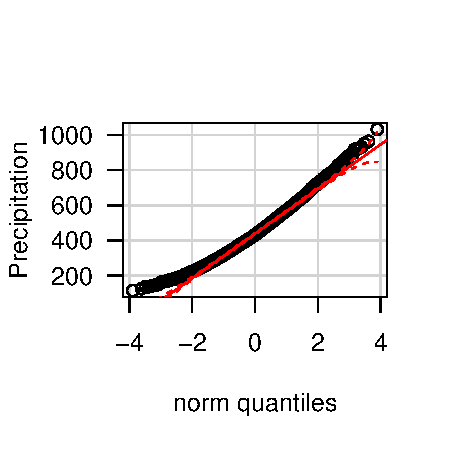
\includegraphics[width=\maxwidth]{figure/1a_qq_seedsamp} 

\end{knitrout}
\end{center} \caption{QQ Plot of Bootstrap Sampling Distribution of Seeded Data.} \end{figure}

\begin{itemize}
\item Seeded Bootsrap Sample Distribtion:  The sampled distribution is unimodal, skewed right, and contains outliers.  The mean of the data is near the mean.  The QQ plot of the sample data shows they are not normally distributed, as more than 5\% of the sample data are outiside of the limits.
\end{itemize}

%%%%%%%%%%%%%%%%%%%%%%%%%%
%% PROB 1 B
%%%%%%%%%%%%%%%%%%%%%%%%%%
\subsection{(10 pts) Repeat the previous question for the log-transformed data.}

\begin{figure}[H]  \begin{center}
\begin{knitrout}
\definecolor{shadecolor}{rgb}{0.969, 0.969, 0.969}\color{fgcolor}\begin{kframe}
\begin{alltt}
\hlcom{# histogram of LogUS Precip}
\hlstd{Precip.hist} \hlkwb{<-} \hlkwd{ggplot}\hlstd{(d1,} \hlkwd{aes}\hlstd{(}\hlkwc{x} \hlstd{= LogUS))}
\hlstd{Precip.hist} \hlkwb{<-} \hlstd{Precip.hist} \hlopt{+} \hlkwd{geom_histogram}\hlstd{(}\hlkwc{binwidth} \hlstd{=} \hlnum{1}\hlstd{,}\hlkwc{color} \hlstd{=} \hlstr{"black"}\hlstd{,}
                                            \hlkwc{fill} \hlstd{=} \hlstr{"white"}\hlstd{)}
\hlstd{Precip.hist} \hlkwb{<-} \hlstd{Precip.hist} \hlopt{+} \hlkwd{labs}\hlstd{(}\hlkwc{title} \hlstd{=} \hlstr{"Precipitation, Log Unseeded"}\hlstd{)}

\hlcom{# boxplot of Log Unseeded Precip}
\hlstd{Precip.box} \hlkwb{<-} \hlkwd{ggplot}\hlstd{(d1,} \hlkwd{aes}\hlstd{(}\hlkwc{x} \hlstd{=} \hlstr{"Precipitation"}\hlstd{,}\hlkwc{y} \hlstd{= LogUS))} \hlcom{# boxplot of Precip}
\hlstd{Precip.box} \hlkwb{<-} \hlstd{Precip.box} \hlopt{+} \hlkwd{geom_boxplot}\hlstd{()}
\hlstd{Precip.box} \hlkwb{<-} \hlstd{Precip.box} \hlopt{+} \hlkwd{coord_flip}\hlstd{()}
\hlstd{Precip.box} \hlkwb{<-} \hlstd{Precip.box} \hlopt{+} \hlkwd{stat_summary}\hlstd{(}\hlkwc{fun.y} \hlstd{= mean,} \hlkwc{geom} \hlstd{=} \hlstr{"point"}\hlstd{,}
                                        \hlkwc{shape} \hlstd{=} \hlnum{3}\hlstd{,} \hlkwc{size} \hlstd{=} \hlnum{4}\hlstd{)}

\hlcom{# plot histogram and boxplot}
\hlkwd{grid.arrange}\hlstd{(Precip.hist, Precip.box,} \hlkwc{nrow} \hlstd{=} \hlnum{2}\hlstd{)}
\end{alltt}
\end{kframe}
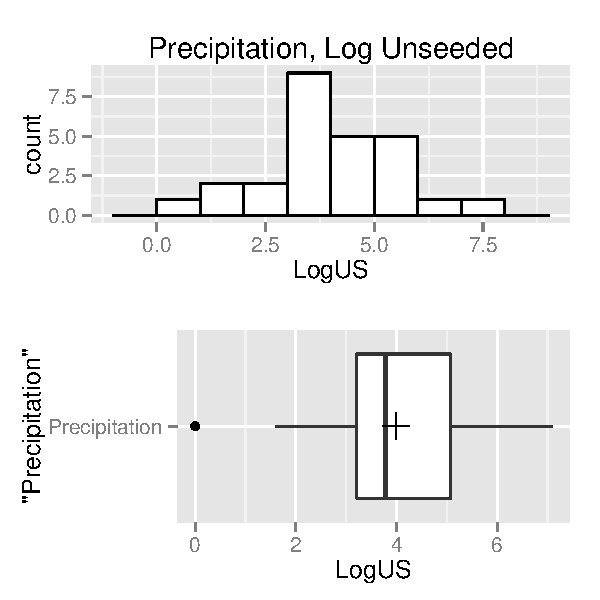
\includegraphics[width=\maxwidth]{figure/1a_data_LogUS} 

\end{knitrout}
\end{center} \caption{Histogram and Boxplot of Log-Transformed Unseeded Data Distribution.} \end{figure}


\begin{figure}[H]  \begin{center} \vspace{-0.45in}
\begin{knitrout}
\definecolor{shadecolor}{rgb}{0.969, 0.969, 0.969}\color{fgcolor}\begin{kframe}
\begin{alltt}
\hlcom{# qq plot for LogUS data}
\hlkwd{qqPlot}\hlstd{(d1}\hlopt{$}\hlstd{LogUS,} \hlkwc{las} \hlstd{=} \hlnum{1}\hlstd{,} \hlkwc{id.n} \hlstd{=} \hlnum{0}\hlstd{,} \hlkwc{id.cex} \hlstd{=} \hlnum{1}\hlstd{,} \hlkwc{lwd} \hlstd{=} \hlnum{1}\hlstd{,} \hlkwc{ylab} \hlstd{=} \hlstr{"Precipitation"}\hlstd{)}
\end{alltt}
\end{kframe}
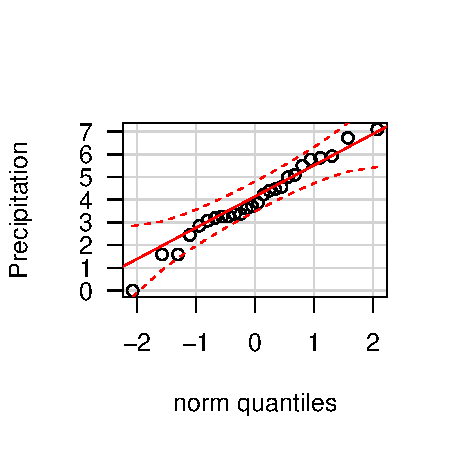
\includegraphics[width=\maxwidth]{figure/1a_qq_LogUS} 

\end{knitrout}
\end{center}\caption{QQ Plot of Log-Transformed Unseeded Data Distribution.} \end{figure}


\begin{itemize}
\item Log-Transformed Unseeded Data Distribtion:  The data distribution is unimodal, normal, and contains one outlier.  The mean of the data is inside of the IQR.  The distribution does not appear to be affected by the one sidedness of the untransformed data. The QQ plot of the data shows  the data are normally distributed, as they closely follow the line representing normality and none of the data are outside of the limits.
\end{itemize}

\begin{figure}[H]  \begin{center}
\begin{knitrout}
\definecolor{shadecolor}{rgb}{0.969, 0.969, 0.969}\color{fgcolor}\begin{kframe}
\begin{alltt}
\hlstd{LogUS.samp} \hlkwb{<-} \hlkwd{bs.one.samp.dist}\hlstd{(d1}\hlopt{$}\hlstd{LogUS)}  \hlcom{# bootstrap of LogUS data}
\end{alltt}
\end{kframe}
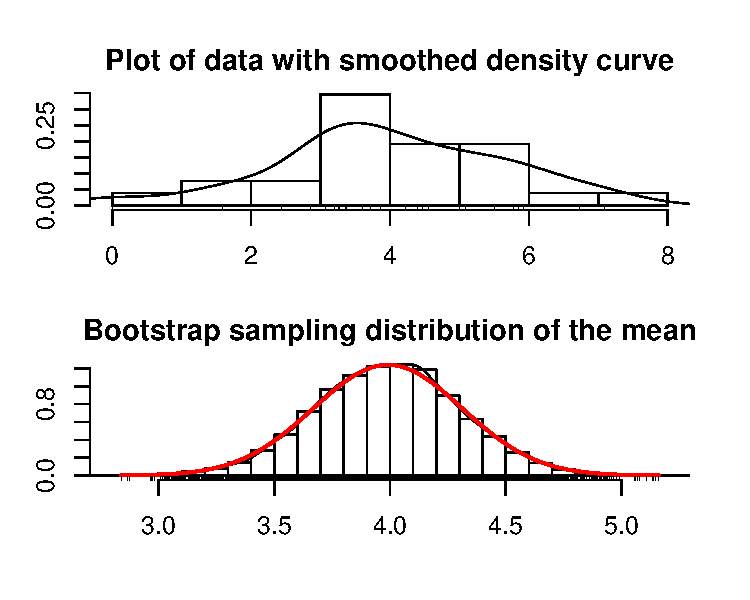
\includegraphics[width=\maxwidth]{figure/1a_boot_LogUS} 
\begin{kframe}\begin{alltt}
\hlstd{LogUS.samp.df} \hlkwb{<-} \hlkwd{data.frame}\hlstd{(LogUS.samp)}
\end{alltt}
\end{kframe}
\end{knitrout}
\end{center} \caption{Resuts of Sampling Distribution from Bootstrap Function of Log-Transformed Unseeded Data.} \end{figure}

\begin{figure}[H]  \begin{center} \vspace{-0.25in}
\begin{knitrout}
\definecolor{shadecolor}{rgb}{0.969, 0.969, 0.969}\color{fgcolor}\begin{kframe}
\begin{alltt}
\hlcom{# histogram of LogUS Precip}
\hlstd{Samp.hist.LogUS} \hlkwb{<-} \hlkwd{ggplot}\hlstd{(LogUS.samp.df,} \hlkwd{aes}\hlstd{(}\hlkwc{x} \hlstd{= LogUS.samp))}
\hlstd{Samp.hist.LogUS} \hlkwb{<-} \hlstd{Samp.hist.LogUS} \hlopt{+} \hlkwd{geom_histogram}\hlstd{(}\hlkwc{binwidth} \hlstd{=} \hlnum{.25}\hlstd{,}\hlkwc{color} \hlstd{=} \hlstr{"black"}\hlstd{,}
                                            \hlkwc{fill} \hlstd{=} \hlstr{"white"}\hlstd{)}
\hlstd{Samp.hist.LogUS} \hlkwb{<-} \hlstd{Samp.hist.LogUS} \hlopt{+}
  \hlkwd{labs}\hlstd{(}\hlkwc{title} \hlstd{=} \hlstr{"Precipitation, Bootstrap Sample of Log Unseeded"}\hlstd{)}

\hlcom{# boxplot of LogUS Precip}
\hlstd{Samp.box.LogUS} \hlkwb{<-} \hlkwd{ggplot}\hlstd{(LogUS.samp.df,} \hlkwd{aes}\hlstd{(}\hlkwc{x} \hlstd{=} \hlstr{"Precipitation"}\hlstd{,}\hlkwc{y} \hlstd{= LogUS.samp))}
\hlstd{Samp.box.LogUS} \hlkwb{<-} \hlstd{Samp.box.LogUS} \hlopt{+} \hlkwd{geom_boxplot}\hlstd{()}
\hlstd{Samp.box.LogUS} \hlkwb{<-} \hlstd{Samp.box.LogUS} \hlopt{+} \hlkwd{coord_flip}\hlstd{()}
\hlstd{Samp.box.LogUS} \hlkwb{<-} \hlstd{Samp.box.LogUS} \hlopt{+} \hlkwd{stat_summary}\hlstd{(}\hlkwc{fun.y} \hlstd{= mean,} \hlkwc{geom} \hlstd{=} \hlstr{"point"}\hlstd{,}
                                        \hlkwc{shape} \hlstd{=} \hlnum{3}\hlstd{,} \hlkwc{size} \hlstd{=} \hlnum{4}\hlstd{)}

\hlcom{# plot histogram and boxplot}
\hlkwd{grid.arrange}\hlstd{(Samp.hist.LogUS, Samp.box.LogUS,} \hlkwc{nrow} \hlstd{=} \hlnum{2}\hlstd{)}
\end{alltt}
\end{kframe}
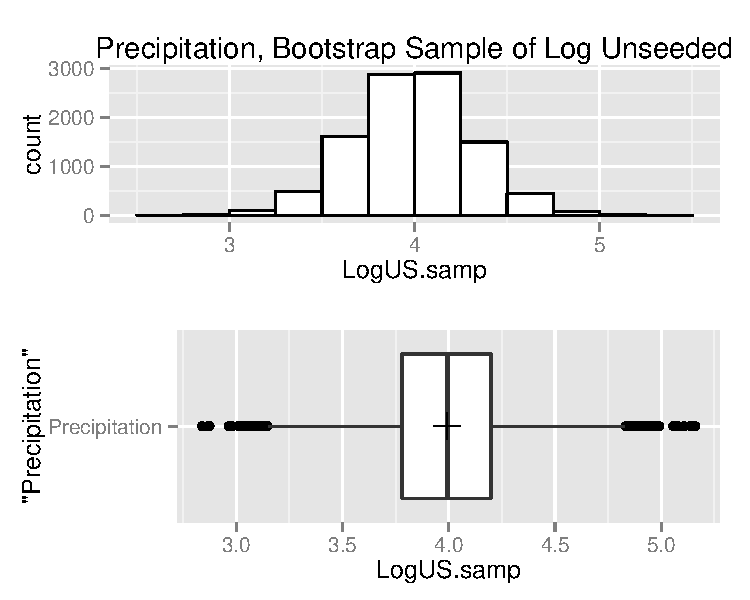
\includegraphics[width=\maxwidth]{figure/1a_box_LogUS} 

\end{knitrout}
\end{center}\caption{Histogram and Boxplot of Bootstrap Sample Distribution of Log-Transformed Unseeded Data.} \end{figure}

\begin{figure}[H]  \begin{center}
\begin{knitrout}
\definecolor{shadecolor}{rgb}{0.969, 0.969, 0.969}\color{fgcolor}\begin{kframe}
\begin{alltt}
\hlcom{# qq plot for bootstrap sampling distribution of LogUS data}
\hlkwd{qqPlot}\hlstd{(LogUS.samp,} \hlkwc{las} \hlstd{=} \hlnum{1}\hlstd{,} \hlkwc{id.n} \hlstd{=} \hlnum{0}\hlstd{,} \hlkwc{id.cex} \hlstd{=} \hlnum{1}\hlstd{,} \hlkwc{lwd} \hlstd{=} \hlnum{1}\hlstd{,} \hlkwc{ylab} \hlstd{=} \hlstr{"Precipitation"}\hlstd{)}
\end{alltt}
\end{kframe}
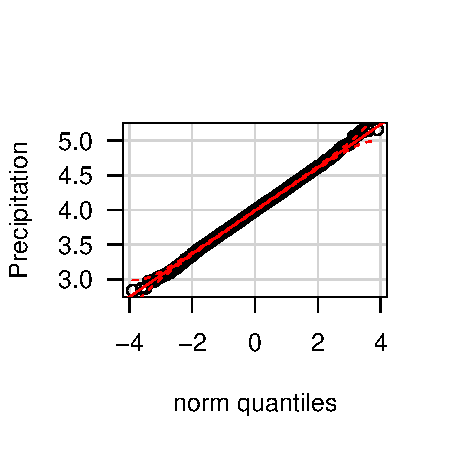
\includegraphics[width=\maxwidth]{figure/1a_qq_LogUSsamp} 

\end{knitrout}
\end{center} \caption{QQ Plot of Bootstrap Sampling Distribution of Log-Transformed Unseeded Data.} \end{figure}

\begin{itemize}
\item Log-Transformed Unseeded Bootsrap Sample Distribtion:  The sampled distribution is unimodal, normal, and contains outliers.  The mean of the data is nearly the median.  The distribution does not appear to be affected by the one sidedness of the untransformed data. The QQ plot of the data shows  the data are normally distributed, as they closely follow the line representing normality.
\end{itemize}

%% ==========================================
%% Log seeded data
%% ==========================================

\begin{knitrout}
\definecolor{shadecolor}{rgb}{0.969, 0.969, 0.969}\color{fgcolor}\begin{kframe}
\begin{alltt}
\hlcom{# histogram of Log Seeded Precip}
\hlstd{Precip.hist.LogS} \hlkwb{<-} \hlkwd{ggplot}\hlstd{(d1,} \hlkwd{aes}\hlstd{(}\hlkwc{x} \hlstd{= LogS))}
\hlstd{Precip.hist.LogS} \hlkwb{<-} \hlstd{Precip.hist.LogS} \hlopt{+} \hlkwd{geom_histogram}\hlstd{(}\hlkwc{binwidth} \hlstd{=} \hlnum{1}\hlstd{,}\hlkwc{color} \hlstd{=} \hlstr{"black"}\hlstd{,}
                                            \hlkwc{fill} \hlstd{=} \hlstr{"white"}\hlstd{)}
\hlstd{Precip.hist.LogS} \hlkwb{<-} \hlstd{Precip.hist.LogS} \hlopt{+} \hlkwd{labs}\hlstd{(}\hlkwc{title} \hlstd{=} \hlstr{"Precipitation, Log Seeded"}\hlstd{)}

\hlcom{# boxplot of Log Seeded Precip}
\hlstd{Precip.box.LogS} \hlkwb{<-} \hlkwd{ggplot}\hlstd{(d1,} \hlkwd{aes}\hlstd{(}\hlkwc{x} \hlstd{=} \hlstr{"Precipitation"}\hlstd{,}\hlkwc{y} \hlstd{= LogS))} \hlcom{# boxplot of Precip}
\hlstd{Precip.box.LogS} \hlkwb{<-} \hlstd{Precip.box.LogS} \hlopt{+} \hlkwd{geom_boxplot}\hlstd{()}
\hlstd{Precip.box.LogS} \hlkwb{<-} \hlstd{Precip.box.LogS} \hlopt{+} \hlkwd{coord_flip}\hlstd{()}
\hlstd{Precip.box.LogS} \hlkwb{<-} \hlstd{Precip.box.LogS} \hlopt{+} \hlkwd{stat_summary}\hlstd{(}\hlkwc{fun.y} \hlstd{= mean,} \hlkwc{geom} \hlstd{=} \hlstr{"point"}\hlstd{,}
                                        \hlkwc{shape} \hlstd{=} \hlnum{3}\hlstd{,} \hlkwc{size} \hlstd{=} \hlnum{4}\hlstd{)}
\end{alltt}
\end{kframe}
\end{knitrout}

\begin{figure}[H]  \begin{center}
\begin{knitrout}
\definecolor{shadecolor}{rgb}{0.969, 0.969, 0.969}\color{fgcolor}\begin{kframe}
\begin{alltt}
\hlcom{# plot histogram and boxplot}
\hlkwd{grid.arrange}\hlstd{(Precip.hist.LogS, Precip.box.LogS,} \hlkwc{nrow} \hlstd{=} \hlnum{2}\hlstd{)}
\end{alltt}
\end{kframe}
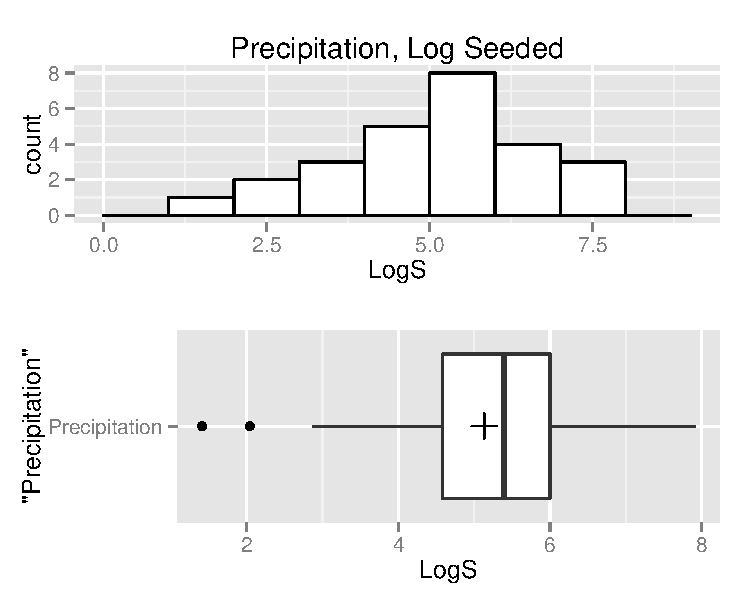
\includegraphics[width=\maxwidth]{figure/1a_data_LogS_plot} 

\end{knitrout}
\end{center} \caption{Histogram and Boxplot of Log-Transformed Seeded Data Distribution.} \end{figure}


\begin{figure}[H]  \begin{center} \vspace{-0.45in}
\begin{knitrout}
\definecolor{shadecolor}{rgb}{0.969, 0.969, 0.969}\color{fgcolor}\begin{kframe}
\begin{alltt}
\hlcom{# qq plot for Log Seeded data}
\hlkwd{qqPlot}\hlstd{(d1}\hlopt{$}\hlstd{LogS,} \hlkwc{las} \hlstd{=} \hlnum{1}\hlstd{,} \hlkwc{id.n} \hlstd{=} \hlnum{0}\hlstd{,} \hlkwc{id.cex} \hlstd{=} \hlnum{1}\hlstd{,} \hlkwc{lwd} \hlstd{=} \hlnum{1}\hlstd{,} \hlkwc{ylab} \hlstd{=} \hlstr{"Precipitation"}\hlstd{)}
\end{alltt}
\end{kframe}
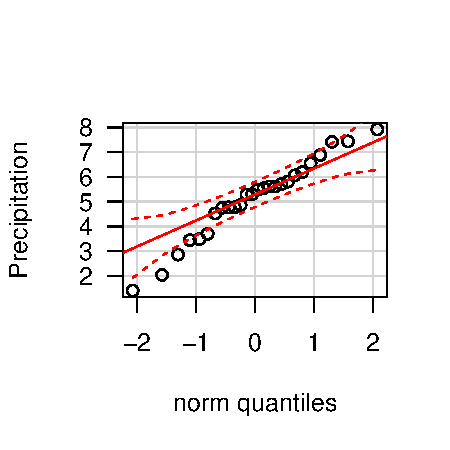
\includegraphics[width=\maxwidth]{figure/1a_qq_LogS} 

\end{knitrout}
\end{center}\caption{QQ Plot of Log-Transformed Seeded Data Distribution.} \end{figure}


\begin{itemize}
\item Log-Transformed Seeded Data Distribtion:  The distribution is unimodal, has equilength tails, and contains two outliers.  The mean of the data is inside the IQR.  The QQ plot of the data shows  the data are not normally distributed, as over 25\% of the data are outside of the CI limits of a normal distribution.  If these data were normal, I would exect only 5\% to be beyone these limits.
\end{itemize}

\begin{figure}[H]  \begin{center}
\begin{knitrout}
\definecolor{shadecolor}{rgb}{0.969, 0.969, 0.969}\color{fgcolor}\begin{kframe}
\begin{alltt}
\hlstd{LogS.samp} \hlkwb{<-} \hlkwd{bs.one.samp.dist}\hlstd{(d1}\hlopt{$}\hlstd{LogS)}  \hlcom{# bootstrap of Log seeded data}
\end{alltt}
\end{kframe}
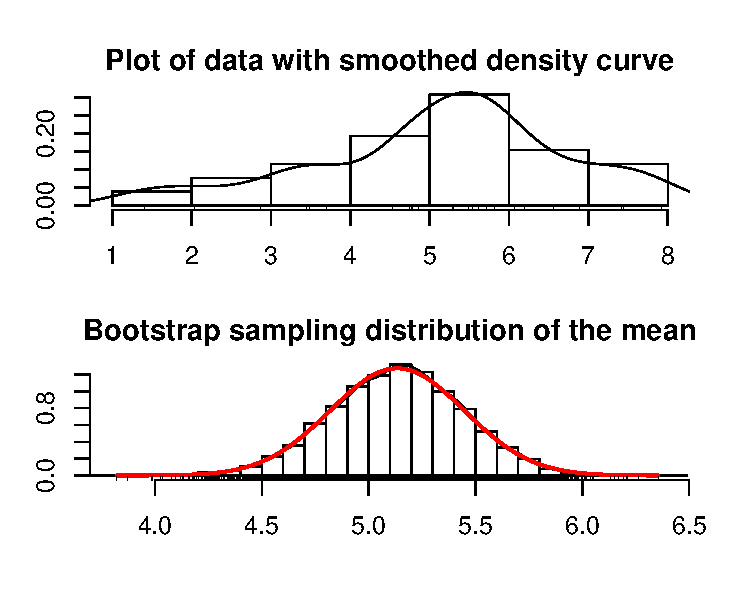
\includegraphics[width=\maxwidth]{figure/1a_boot_LogS} 

\end{knitrout}
\end{center} \caption{Resuts of Sampling Distribution from Bootstrap Function of Log-Transformed Seeded Data.}
\end{figure}

\begin{knitrout}
\definecolor{shadecolor}{rgb}{0.969, 0.969, 0.969}\color{fgcolor}\begin{kframe}
\begin{alltt}
\hlcom{# histogram of LogUS Precip}
\hlstd{LogS.samp.df} \hlkwb{<-} \hlkwd{data.frame}\hlstd{(LogS.samp)}
\hlstd{Samp.hist.LogS} \hlkwb{<-} \hlkwd{ggplot}\hlstd{(LogS.samp.df,} \hlkwd{aes}\hlstd{(}\hlkwc{x} \hlstd{= LogS.samp))}
\hlstd{Samp.hist.LogS} \hlkwb{<-} \hlstd{Samp.hist.LogS} \hlopt{+} \hlkwd{geom_histogram}\hlstd{(}\hlkwc{binwidth} \hlstd{=} \hlnum{.25}\hlstd{,}\hlkwc{color} \hlstd{=} \hlstr{"black"}\hlstd{,}
                                            \hlkwc{fill} \hlstd{=} \hlstr{"white"}\hlstd{)}
\hlstd{Samp.hist.LogS} \hlkwb{<-} \hlstd{Samp.hist.LogS} \hlopt{+}
  \hlkwd{labs}\hlstd{(}\hlkwc{title} \hlstd{=} \hlstr{"Precipitation, Bootstrap Sample of Log Seeded"}\hlstd{)}

\hlcom{# boxplot of Log Seeded Precip}
\hlstd{Samp.box.LogS} \hlkwb{<-} \hlkwd{ggplot}\hlstd{(LogS.samp.df,}
                        \hlkwd{aes}\hlstd{(}\hlkwc{x} \hlstd{=} \hlstr{"Precipitation"}\hlstd{,}\hlkwc{y} \hlstd{= LogS.samp))} \hlcom{# boxplot of Precip}
\hlstd{Samp.box.LogS} \hlkwb{<-} \hlstd{Samp.box.LogS} \hlopt{+} \hlkwd{geom_boxplot}\hlstd{()}
\hlstd{Samp.box.LogS} \hlkwb{<-} \hlstd{Samp.box.LogS} \hlopt{+} \hlkwd{coord_flip}\hlstd{()}
\hlstd{Samp.box.LogS} \hlkwb{<-} \hlstd{Samp.box.LogS} \hlopt{+} \hlkwd{stat_summary}\hlstd{(}\hlkwc{fun.y} \hlstd{= mean,} \hlkwc{geom} \hlstd{=} \hlstr{"point"}\hlstd{,}
                                        \hlkwc{shape} \hlstd{=} \hlnum{3}\hlstd{,} \hlkwc{size} \hlstd{=} \hlnum{4}\hlstd{)}
\end{alltt}
\end{kframe}
\end{knitrout}

\begin{figure}[H]  \begin{center} \vspace{-0.45in}
\begin{knitrout}
\definecolor{shadecolor}{rgb}{0.969, 0.969, 0.969}\color{fgcolor}\begin{kframe}
\begin{alltt}
\hlcom{# plot histogram and boxplot}
\hlkwd{grid.arrange}\hlstd{(Samp.hist.LogS, Samp.box.LogS,} \hlkwc{nrow} \hlstd{=} \hlnum{2}\hlstd{)}
\end{alltt}
\end{kframe}
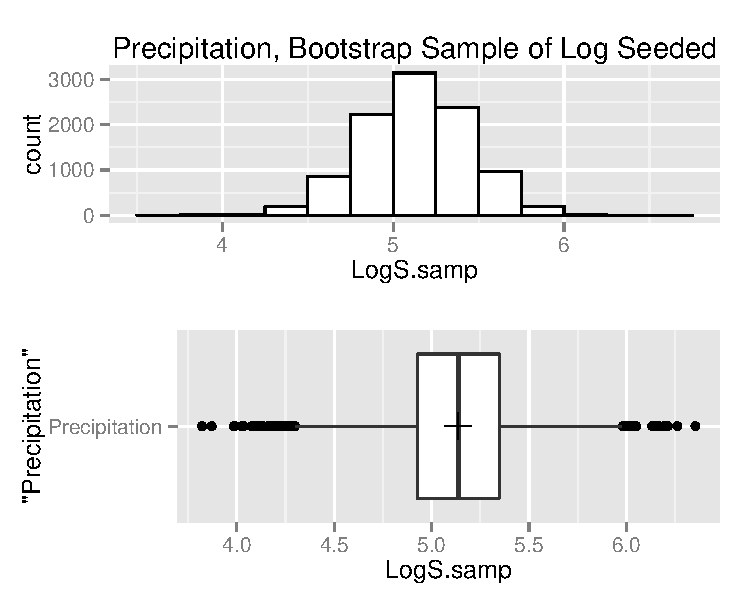
\includegraphics[width=\maxwidth]{figure/1a_box_LogS_plot} 

\end{knitrout}
\end{center}\caption{Histogram and Boxplot of Bootstrap Sample Distribution of Log-Transformed Seeded Data.} \end{figure}

\begin{figure}[H]  \begin{center}
\begin{knitrout}
\definecolor{shadecolor}{rgb}{0.969, 0.969, 0.969}\color{fgcolor}\begin{kframe}
\begin{alltt}
\hlcom{# qq plot for bootstrap sampling distribution of Log seeded data}
\hlkwd{qqPlot}\hlstd{(LogS.samp,} \hlkwc{las} \hlstd{=} \hlnum{1}\hlstd{,} \hlkwc{id.n} \hlstd{=} \hlnum{0}\hlstd{,} \hlkwc{id.cex} \hlstd{=} \hlnum{1}\hlstd{,} \hlkwc{lwd} \hlstd{=} \hlnum{1}\hlstd{,} \hlkwc{ylab} \hlstd{=} \hlstr{"Precipitation"}\hlstd{)}
\end{alltt}
\end{kframe}
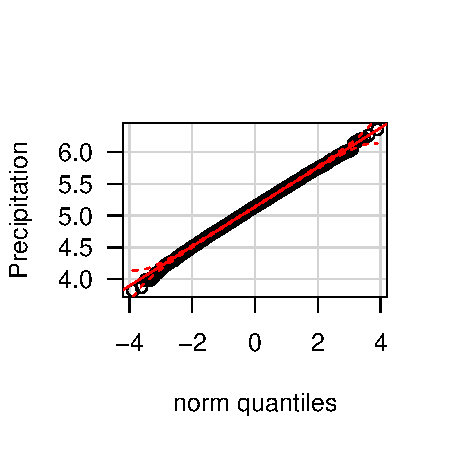
\includegraphics[width=\maxwidth]{figure/1a_qq_LogSsamp} 

\end{knitrout}
\end{center} \caption{QQ Plot of Bootstrap Sampling Distribution of Log-Transformed Seeded Data.} \end{figure}

\begin{itemize}
\item Log-Transformed Seeded Bootsrap Sample Distribtion:  The sampled distribution is unimodal, normal, and contains outliers.  The tails are equilength, and the mean of the data is near the mean.  The QQ plot of the sample data shows they are normally distributed.
\end{itemize}

%%%%%%%%%%%%%%%%%%%%%%%%%%
%% PROB 1 C
%%%%%%%%%%%%%%%%%%%%%%%%%%

\subsection{(20 pts) Compare the groups using two-sample t-procedures. Choose the most appropriate scale
(natural or log units) in which to perform this analysis.}

\begin{itemize}
  \item Scale for analysis:  The log-transfered data will be used for the  two sample analysis.  The standard deviation between the two samples varies by less than 3\%; therefore, the pooled variance method.
  \item Definition of Population Parameters: $\mu = \mu_1 - \mu_2 = $  The population parameter is  the difference in the population mean precipitation volume between unseeded and seeded clouds.
  \item Hypothesis:  Is it plausible that the difference in the population mean precipitation volume is different from zero.  In notation:  $H_0: \mu_1 - \mu_2 = 0$ versus $H_A: \mu_1 - \mu_2 \ne 0$

\begin{knitrout}
\definecolor{shadecolor}{rgb}{0.969, 0.969, 0.969}\color{fgcolor}\begin{kframe}
\begin{alltt}
\hlcom{# summary of statistics}
\hlstd{m1} \hlkwb{<-} \hlkwd{mean}\hlstd{(LogUS)}
\hlstd{s1} \hlkwb{<-} \hlkwd{sd}\hlstd{(LogUS)}
\hlstd{n1} \hlkwb{<-} \hlkwd{length}\hlstd{(LogUS)}
\hlstd{m2} \hlkwb{<-} \hlkwd{mean}\hlstd{(LogS)}
\hlstd{s2} \hlkwb{<-} \hlkwd{sd}\hlstd{(LogS)}
\hlstd{n2} \hlkwb{<-} \hlkwd{length}\hlstd{(LogS)}

\hlkwd{c}\hlstd{(m1, s1, n1)} \hlcom{#Unseeded statistics}
\end{alltt}
\begin{verbatim}
## [1]  3.990  1.642 26.000
\end{verbatim}
\begin{alltt}
\hlkwd{c}\hlstd{(m2, s2, n2)} \hlcom{#Seeded Statistics}
\end{alltt}
\begin{verbatim}
## [1]  5.134  1.600 26.000
\end{verbatim}
\begin{alltt}
\hlcom{# Two sample T Test test with pooled variance}
\hlstd{d1.c.t} \hlkwb{<-} \hlkwd{t.test}\hlstd{(LogUS, LogS,} \hlkwc{var.equal} \hlstd{=} \hlnum{TRUE}\hlstd{)}
\hlstd{d1.c.t}
\end{alltt}
\begin{verbatim}
## 
## 	Two Sample t-test
## 
## data:  LogUS and LogS
## t = -2.544, df = 50, p-value = 0.01408
## alternative hypothesis: true difference in means is not equal to 0
## 95 percent confidence interval:
##  -2.0467 -0.2409
## sample estimates:
## mean of x mean of y 
##     3.990     5.134
\end{verbatim}
\end{kframe}
\end{knitrout}

\item  Summary:  The pooled analysis suggests that the difference in the mean precipitation volume is different than zero.  The t-statistic was -2.5 and two-sided p-value was $1.4 \times 10^{-2}$ therefore, because the p-value is less than 0.05, I reject the Null hypothesis ($H_0: \mu_1 - \mu_2 = 0$) in favor of the Alternative hypothesis ($H_A: \mu_1 - \mu_2 \ne 0$).  The Difference in the population mean precipitation volume between the unseeded and seeded clouds are different.  \

With 95\% confidence, the difference in the poulation mean precipitation volume ($\mu_1 - \mu_2$) is between -2.0 and -0.2.  That is, I am $95\%$ confident that the population mean precipitation volume for seeded clouds $\mu_2$ exceeds the population mean precipiation volume for unseeded clouds $\mu_1$ by betwen 0.2 and 2.0 units.

\begin{figure}[H]  \begin{center} \vspace{-0.45in}
\begin{knitrout}
\definecolor{shadecolor}{rgb}{0.969, 0.969, 0.969}\color{fgcolor}\begin{kframe}
\begin{alltt}
\hlcom{#### Visual comparison of whether sampling distribution is close to Normal via Bootstrap}
\hlkwd{bs.two.samp.diff.dist}\hlstd{(LogS, LogUS)}
\end{alltt}
\end{kframe}
\includegraphics[width=\maxwidth]{figure/1c_bootstrap} 

\end{knitrout}
\end{center} \caption{Bootstrap Sampling Distribution of Pooled Log-Transformed Precipitation Data.} \end{figure}

  \item Assumptions:  The pooled variance method assumes the populations have normal frequency curves, with equal population standard deviations.  As shown above, the distribution of difference in means is very close to normal.
\end{itemize}
%%%%%%%%%%%%%%%%%%%%%%%%%%%%%%%%%%%%%%%%%
%%%%%%%%%%%%%%%%%%%%%%%%%%%%%%%%%%%%%%%%%
%%% problem 2
%%%%%%%%%%%%%%%%%%%%%%%%%%%%%%%%%%%%%%%%%
%%%%%%%%%%%%%%%%%%%%%%%%%%%%%%%%%%%%%%%%%

\section{Acid}
\begin{knitrout}
\definecolor{shadecolor}{rgb}{0.969, 0.969, 0.969}\color{fgcolor}\begin{kframe}
\begin{alltt}
\hlstd{d2} \hlkwb{<-} \hlkwd{read.csv}\hlstd{(}\hlstr{"http://statacumen.com/teach/ADA1/ADA1_HW_02_F14-3.csv"}\hlstd{)}
\hlstd{acid1} \hlkwb{<-} \hlkwd{subset}\hlstd{(d2,exper} \hlopt{==}\hlstr{"Acid1"}\hlstd{,} \hlkwc{select} \hlstd{=} \hlkwd{c}\hlstd{(conc,exper))}
\hlstd{acid2} \hlkwb{<-} \hlkwd{subset}\hlstd{(d2,exper} \hlopt{==}\hlstr{"Acid2"}\hlstd{,} \hlkwc{select} \hlstd{=} \hlkwd{c}\hlstd{(conc,exper))}
\end{alltt}
\end{kframe}
\end{knitrout}

The population parameter is the average acidity of the solution in the chemistry class.  The hypothesis is if the class was "biased" and thought the acidity was either less or greater than
it actually was.

\subsection{(10 pts) Check the normality assumption for both experiments as in problem 1 above.}
\subsubsection{Acid 1}

\begin{knitrout}
\definecolor{shadecolor}{rgb}{0.969, 0.969, 0.969}\color{fgcolor}\begin{kframe}
\begin{alltt}
\hlcom{# histogram of acid1}
\hlstd{acid1.hist} \hlkwb{<-} \hlkwd{ggplot}\hlstd{(acid1,} \hlkwd{aes}\hlstd{(}\hlkwc{x} \hlstd{= conc))}
\hlstd{acid1.hist} \hlkwb{<-} \hlstd{acid1.hist} \hlopt{+} \hlkwd{geom_histogram}\hlstd{(}\hlkwc{binwidth} \hlstd{=} \hlnum{.001}\hlstd{)}

\hlcom{# boxplot of acid1}
\hlstd{acid1.box} \hlkwb{<-} \hlkwd{ggplot}\hlstd{(acid1,} \hlkwd{aes}\hlstd{(}\hlkwc{x} \hlstd{=} \hlstr{"Concentration"}\hlstd{,} \hlkwc{y} \hlstd{= conc))} \hlcom{# boxplot of acid1}
\hlstd{acid1.box} \hlkwb{<-} \hlstd{acid1.box} \hlopt{+} \hlkwd{geom_boxplot}\hlstd{()}
\hlstd{acid1.box} \hlkwb{<-} \hlstd{acid1.box} \hlopt{+} \hlkwd{coord_flip}\hlstd{()}
\hlstd{acid1.box} \hlkwb{<-} \hlstd{acid1.box} \hlopt{+} \hlkwd{stat_summary}\hlstd{(}\hlkwc{fun.y} \hlstd{= mean,} \hlkwc{geom} \hlstd{=} \hlstr{"point"}\hlstd{,} \hlkwc{shape} \hlstd{=} \hlnum{3}\hlstd{,} \hlkwc{size} \hlstd{=} \hlnum{2}\hlstd{)}
\end{alltt}
\end{kframe}
\end{knitrout}

\begin{figure}[H]  \begin{center}
\begin{knitrout}
\definecolor{shadecolor}{rgb}{0.969, 0.969, 0.969}\color{fgcolor}\begin{kframe}
\begin{alltt}
\hlcom{# plot histogram and boxplot}
\hlkwd{grid.arrange}\hlstd{(acid1.hist, acid1.box,} \hlkwc{nrow} \hlstd{=} \hlnum{2}\hlstd{)}
\end{alltt}
\end{kframe}
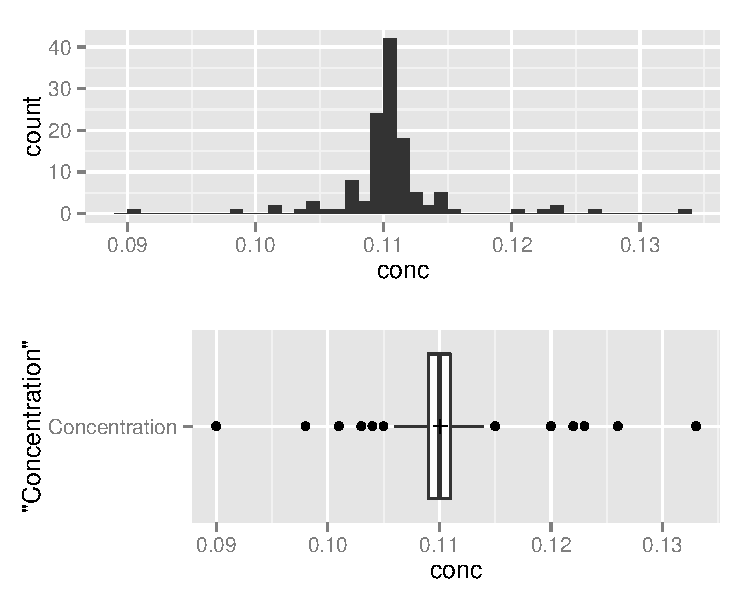
\includegraphics[width=\maxwidth]{figure/2_acid1_boxplot} 

\end{knitrout}
\end{center} \caption{Histogram and Boxplot of Acid 1 Concentration.} \end{figure}

\begin{figure}[H]  \begin{center}
\begin{knitrout}
\definecolor{shadecolor}{rgb}{0.969, 0.969, 0.969}\color{fgcolor}\begin{kframe}
\begin{alltt}
\hlcom{# qq plot for acid 1 concentration data}
\hlkwd{qqPlot}\hlstd{(acid1}\hlopt{$}\hlstd{conc,} \hlkwc{las} \hlstd{=} \hlnum{1}\hlstd{,} \hlkwc{id.n} \hlstd{=} \hlnum{0}\hlstd{,} \hlkwc{id.cex} \hlstd{=} \hlnum{1}\hlstd{,} \hlkwc{lwd} \hlstd{=} \hlnum{1}\hlstd{,} \hlkwc{ylab} \hlstd{=} \hlstr{"Acid 1 Concentration"}\hlstd{)}
\end{alltt}
\end{kframe}
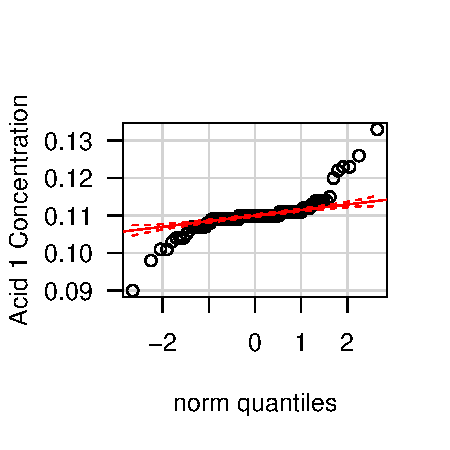
\includegraphics[width=\maxwidth]{figure/2_acid1_qq} 

\end{knitrout}
\end{center}\caption{QQ Plot of Acid 1 Concentration Data Distribution.} \end{figure}

\begin{itemize}
\item Acid 1 Data Distribtion:  The Acid 1 data distribution is unimodal, normal, and contains outliers.  The mean of the data is inside of the IQR and the tails are nearly equal length. The QQ plot of the data shows the are not normally distributed, as they deviate substantially from the line representing normality and more than 5\% of the data are outside of the limits.
\end{itemize}

\begin{figure}[H]  \begin{center}
\begin{knitrout}
\definecolor{shadecolor}{rgb}{0.969, 0.969, 0.969}\color{fgcolor}\begin{kframe}
\begin{alltt}
\hlstd{acid1.boot} \hlkwb{<-} \hlkwd{bs.one.samp.dist}\hlstd{(acid1}\hlopt{$}\hlstd{conc)}      \hlcom{# plot histogram and frequency density curve}
\end{alltt}
\end{kframe}
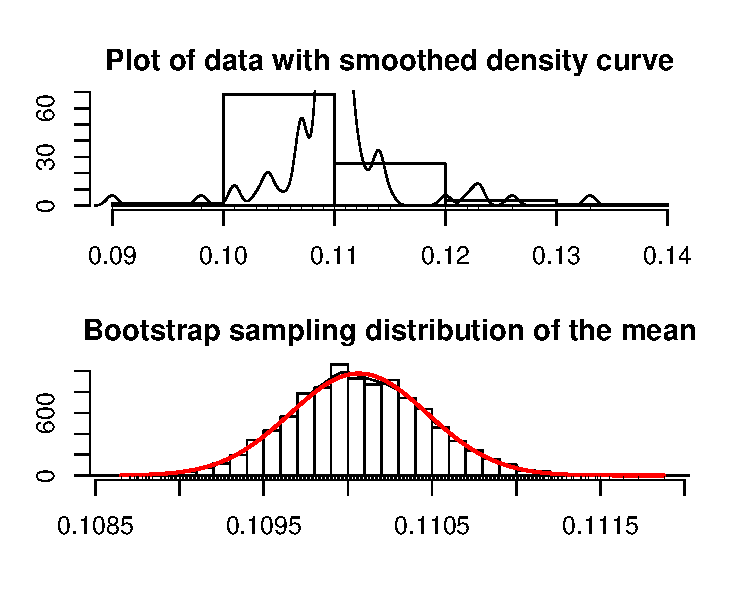
\includegraphics[width=\maxwidth]{figure/2_acid1_boot} 

\end{knitrout}
\end{center}\caption{Bootstrap Sample Distribution of Acid 1.} \end{figure}

\begin{knitrout}
\definecolor{shadecolor}{rgb}{0.969, 0.969, 0.969}\color{fgcolor}\begin{kframe}
\begin{alltt}
\hlstd{acid1.boot.df} \hlkwb{<-} \hlkwd{data.frame}\hlstd{((acid1.boot))}
\hlstd{acid1.boot.df}\hlopt{$}\hlstd{Acid} \hlkwb{<-} \hlkwd{rep}\hlstd{(}\hlstr{"Acid.boot"}\hlstd{,}\hlkwd{length}\hlstd{(acid1.boot))}

\hlcom{# histogram of acid1}
\hlstd{acid1.hist.boot} \hlkwb{<-} \hlkwd{ggplot}\hlstd{(acid1.boot.df,} \hlkwd{aes}\hlstd{(}\hlkwc{x} \hlstd{= X.acid1.boot.))}
\hlstd{acid1.hist.boot} \hlkwb{<-} \hlstd{acid1.hist.boot} \hlopt{+} \hlkwd{geom_histogram}\hlstd{(}\hlkwc{binwidth} \hlstd{=} \hlnum{.0001}\hlstd{)}

\hlcom{# boxplot of acid1}
\hlstd{acid1.box.boot} \hlkwb{<-} \hlkwd{ggplot}\hlstd{(acid1.boot.df,} \hlkwd{aes}\hlstd{(}\hlkwc{x} \hlstd{=} \hlstr{"Concentration"}\hlstd{,} \hlkwc{y} \hlstd{= X.acid1.boot.))} \hlcom{# boxplot of acid1}
\hlstd{acid1.box.boot} \hlkwb{<-} \hlstd{acid1.box.boot} \hlopt{+} \hlkwd{geom_boxplot}\hlstd{()}
\hlstd{acid1.box.boot} \hlkwb{<-} \hlstd{acid1.box.boot} \hlopt{+} \hlkwd{coord_flip}\hlstd{()}
\hlstd{acid1.box.boot} \hlkwb{<-} \hlstd{acid1.box.boot} \hlopt{+} \hlkwd{stat_summary}\hlstd{(}\hlkwc{fun.y} \hlstd{= mean,} \hlkwc{geom} \hlstd{=} \hlstr{"point"}\hlstd{,} \hlkwc{shape} \hlstd{=} \hlnum{3}\hlstd{,} \hlkwc{size} \hlstd{=} \hlnum{2}\hlstd{)}
\end{alltt}
\end{kframe}
\end{knitrout}

\begin{figure}[H]  \begin{center}
\begin{knitrout}
\definecolor{shadecolor}{rgb}{0.969, 0.969, 0.969}\color{fgcolor}\begin{kframe}
\begin{alltt}
\hlcom{# plot histogram and boxplot}
\hlkwd{grid.arrange}\hlstd{(acid1.hist.boot, acid1.box.boot,} \hlkwc{nrow} \hlstd{=} \hlnum{2}\hlstd{)}
\end{alltt}
\end{kframe}
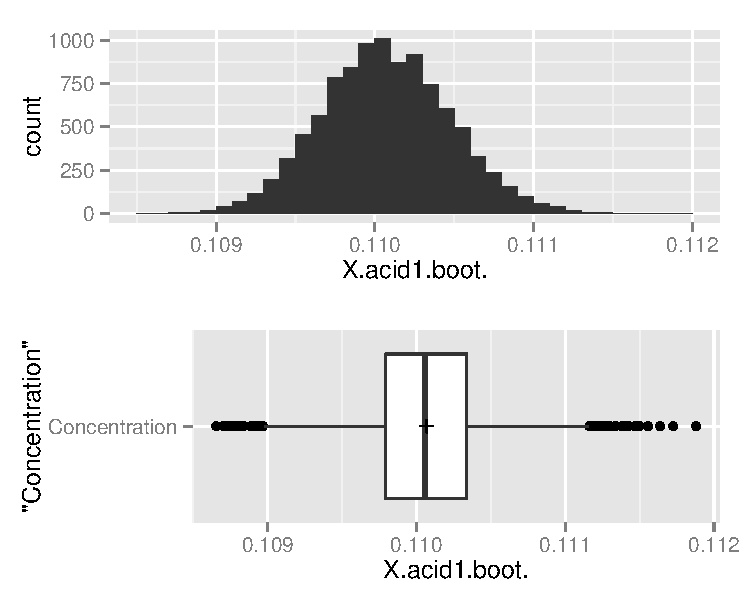
\includegraphics[width=\maxwidth]{figure/2_acid1_bootbox_plot} 

\end{knitrout}
\end{center} \caption{Histogram and Boxplot of Acid 1 Bootstrap Sample Distribution.} \end{figure}

\begin{figure}[H]  \begin{center}
\begin{knitrout}
\definecolor{shadecolor}{rgb}{0.969, 0.969, 0.969}\color{fgcolor}\begin{kframe}
\begin{alltt}
\hlcom{# qq plot for acid 1 concentration data}
\hlkwd{qqPlot}\hlstd{(acid1.boot,} \hlkwc{las} \hlstd{=} \hlnum{1}\hlstd{,} \hlkwc{id.n} \hlstd{=} \hlnum{0}\hlstd{,} \hlkwc{id.cex} \hlstd{=} \hlnum{1}\hlstd{,} \hlkwc{lwd} \hlstd{=} \hlnum{1}\hlstd{)}
\end{alltt}
\end{kframe}
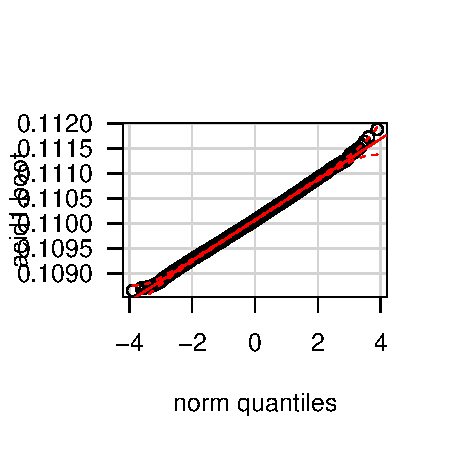
\includegraphics[width=\maxwidth]{figure/2_acid1_qqbott} 

\end{knitrout}
\end{center}\caption{QQ Plot of Acid 1 Concentration Bootstrap Sample Distribution.} \end{figure}

\begin{itemize}
\item Acid 1 Bootstrap Sample Distribtion:  The Acid 1 bootstrap sample distribution is unimodal, normal, and contains outliers.  The mean of the data is inside of the IQR and the tails are nearly equal length. The QQ plot of the data shows the are normally distributed, as they follow the line representing normality very closely.
\end{itemize}

%%%%%%%%%%%%%%
%%% Acid 2
%%%%%%%%%%%%%%
\subsubsection{Acid 2}


\begin{knitrout}
\definecolor{shadecolor}{rgb}{0.969, 0.969, 0.969}\color{fgcolor}\begin{kframe}
\begin{alltt}
\hlcom{# histogram of acid2}
\hlstd{acid2.hist} \hlkwb{<-} \hlkwd{ggplot}\hlstd{(acid2,} \hlkwd{aes}\hlstd{(}\hlkwc{x} \hlstd{= conc))}
\hlstd{acid2.hist} \hlkwb{<-} \hlstd{acid2.hist} \hlopt{+} \hlkwd{geom_histogram}\hlstd{(}\hlkwc{binwidth} \hlstd{=} \hlnum{.001}\hlstd{)}

\hlcom{# boxplot of acid2}
\hlstd{acid2.box} \hlkwb{<-} \hlkwd{ggplot}\hlstd{(acid2,} \hlkwd{aes}\hlstd{(}\hlkwc{x} \hlstd{=} \hlstr{"Concentration"}\hlstd{,} \hlkwc{y} \hlstd{= conc))} \hlcom{# boxplot of acid2}
\hlstd{acid2.box} \hlkwb{<-} \hlstd{acid2.box} \hlopt{+} \hlkwd{geom_boxplot}\hlstd{()}
\hlstd{acid2.box} \hlkwb{<-} \hlstd{acid2.box} \hlopt{+} \hlkwd{coord_flip}\hlstd{()}
\hlstd{acid2.box} \hlkwb{<-} \hlstd{acid2.box} \hlopt{+} \hlkwd{stat_summary}\hlstd{(}\hlkwc{fun.y} \hlstd{= mean,} \hlkwc{geom} \hlstd{=} \hlstr{"point"}\hlstd{,} \hlkwc{shape} \hlstd{=} \hlnum{3}\hlstd{,} \hlkwc{size} \hlstd{=} \hlnum{2}\hlstd{)}
\end{alltt}
\end{kframe}
\end{knitrout}

\begin{figure}[H]  \begin{center}
\begin{knitrout}
\definecolor{shadecolor}{rgb}{0.969, 0.969, 0.969}\color{fgcolor}\begin{kframe}
\begin{alltt}
\hlcom{# plot histogram and boxplot}
\hlkwd{grid.arrange}\hlstd{(acid2.hist, acid2.box,} \hlkwc{nrow} \hlstd{=} \hlnum{2}\hlstd{)}
\end{alltt}
\end{kframe}
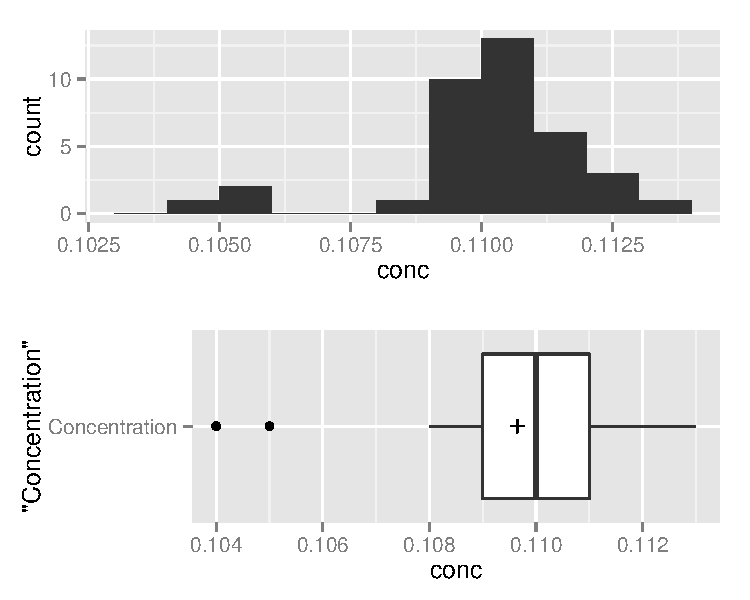
\includegraphics[width=\maxwidth]{figure/2_acid2_box_plot} 

\end{knitrout}
\end{center} \caption{Histogram and Boxplot of Acid 2 Concentration.} \end{figure}

\begin{figure}[H]  \begin{center}
\begin{knitrout}
\definecolor{shadecolor}{rgb}{0.969, 0.969, 0.969}\color{fgcolor}\begin{kframe}
\begin{alltt}
\hlcom{# qq plot for Acid 2 concentration data}
\hlkwd{qqPlot}\hlstd{(acid2}\hlopt{$}\hlstd{conc,} \hlkwc{las} \hlstd{=} \hlnum{1}\hlstd{,} \hlkwc{id.n} \hlstd{=} \hlnum{0}\hlstd{,} \hlkwc{id.cex} \hlstd{=} \hlnum{1}\hlstd{,} \hlkwc{lwd} \hlstd{=} \hlnum{1}\hlstd{,}
       \hlkwc{ylab} \hlstd{=} \hlstr{"Acid 2 Concentration"}\hlstd{)}
\end{alltt}
\end{kframe}
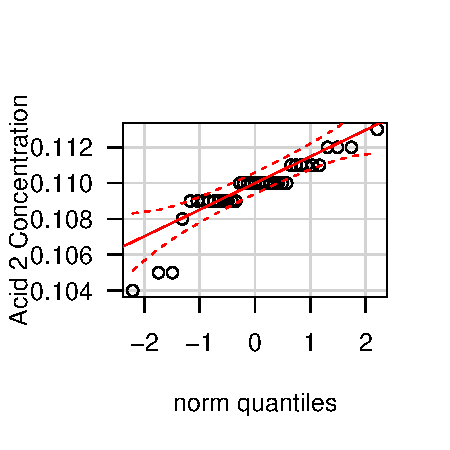
\includegraphics[width=\maxwidth]{figure/2_acid2_qq} 

\end{knitrout}
\end{center}\caption{QQ Plot of Acid 2 Concentration Data Distribution.} \end{figure}

\begin{itemize}
\item Acid 2 Data Distribtion:  The Acid 2 data distribution is unimodal, skewed right, and contains outliers to the left.  The mean of the data is inside of the IQR but the tails are not equal length. The QQ plot of the data shows the are nearly normally distributed, as  8\% of the data are outside of the limits.
\end{itemize}

\begin{figure}[H]  \begin{center}
\begin{knitrout}
\definecolor{shadecolor}{rgb}{0.969, 0.969, 0.969}\color{fgcolor}\begin{kframe}
\begin{alltt}
\hlstd{acid2.boot} \hlkwb{<-} \hlkwd{bs.one.samp.dist}\hlstd{(acid2}\hlopt{$}\hlstd{conc)}  \hlcom{# plot histogram and frequency density curve}
\end{alltt}
\end{kframe}
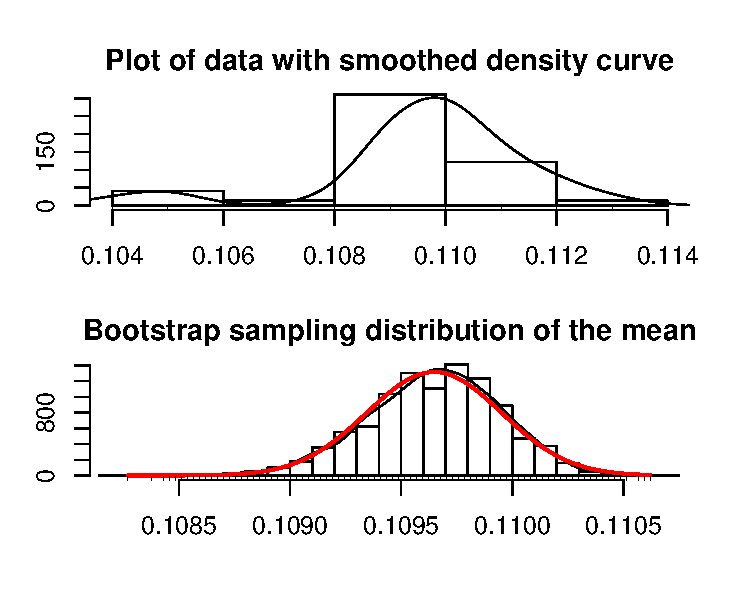
\includegraphics[width=\maxwidth]{figure/2_acid2_boot} 

\end{knitrout}
\end{center}\caption{Bootstrap Sample Distribution of Acid 2.} \end{figure}

\begin{knitrout}
\definecolor{shadecolor}{rgb}{0.969, 0.969, 0.969}\color{fgcolor}\begin{kframe}
\begin{alltt}
\hlstd{acid2.boot.df} \hlkwb{<-} \hlkwd{data.frame}\hlstd{((acid2.boot))}
\hlstd{acid2.boot.df}\hlopt{$}\hlstd{Acid} \hlkwb{<-} \hlkwd{rep}\hlstd{(}\hlstr{"Acid.boot"}\hlstd{,}\hlkwd{length}\hlstd{(acid2.boot))}

\hlcom{# histogram of acid2}
\hlstd{acid2.hist.boot} \hlkwb{<-} \hlkwd{ggplot}\hlstd{(acid2.boot.df,} \hlkwd{aes}\hlstd{(}\hlkwc{x} \hlstd{= X.acid2.boot.))}
\hlstd{acid2.hist.boot} \hlkwb{<-} \hlstd{acid2.hist.boot} \hlopt{+} \hlkwd{geom_histogram}\hlstd{(}\hlkwc{binwidth} \hlstd{=} \hlnum{.0001}\hlstd{)}

\hlcom{# boxplot of acid2}
\hlstd{acid2.box.boot} \hlkwb{<-} \hlkwd{ggplot}\hlstd{(acid2.boot.df,} \hlkwd{aes}\hlstd{(}\hlkwc{x} \hlstd{=} \hlstr{"Concentration"}\hlstd{,} \hlkwc{y} \hlstd{= X.acid2.boot.))}
\hlstd{acid2.box.boot} \hlkwb{<-} \hlstd{acid2.box.boot} \hlopt{+} \hlkwd{geom_boxplot}\hlstd{()}
\hlstd{acid2.box.boot} \hlkwb{<-} \hlstd{acid2.box.boot} \hlopt{+} \hlkwd{coord_flip}\hlstd{()}
\hlstd{acid2.box.boot} \hlkwb{<-} \hlstd{acid2.box.boot} \hlopt{+} \hlkwd{stat_summary}\hlstd{(}\hlkwc{fun.y} \hlstd{= mean,} \hlkwc{geom} \hlstd{=} \hlstr{"point"}\hlstd{,}
                                                \hlkwc{shape} \hlstd{=} \hlnum{3}\hlstd{,} \hlkwc{size} \hlstd{=} \hlnum{2}\hlstd{)}
\end{alltt}
\end{kframe}
\end{knitrout}

\begin{figure}[H]  \begin{center} \vspace{-0.45in}
\begin{knitrout}
\definecolor{shadecolor}{rgb}{0.969, 0.969, 0.969}\color{fgcolor}\begin{kframe}
\begin{alltt}
\hlcom{# plot histogram and boxplot}
\hlkwd{grid.arrange}\hlstd{(acid2.hist.boot, acid2.box.boot,} \hlkwc{nrow} \hlstd{=} \hlnum{2}\hlstd{)}
\end{alltt}
\end{kframe}
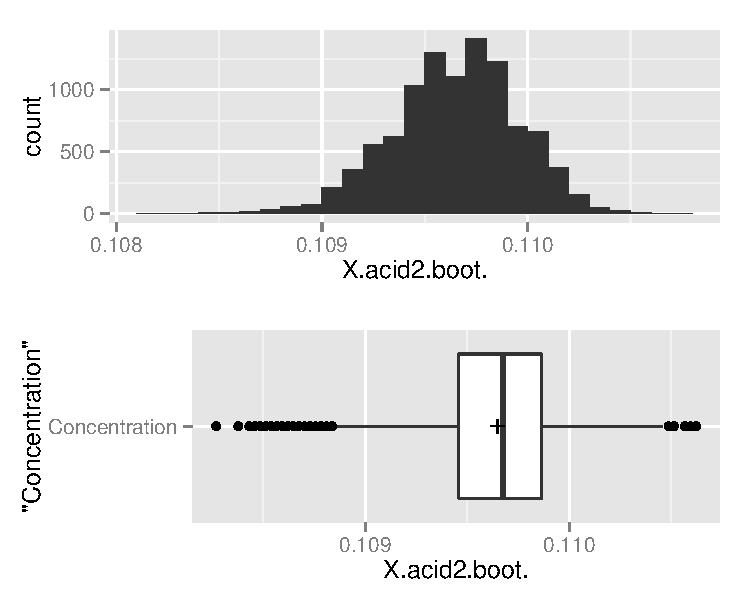
\includegraphics[width=\maxwidth]{figure/2_acid2_bootbox_plot} 

\end{knitrout}
\end{center} \caption{Histogram and Boxplot of Acid 2 Bootstrap Sample Distribution.} \end{figure}

\begin{figure}[H]  \begin{center}
\begin{knitrout}
\definecolor{shadecolor}{rgb}{0.969, 0.969, 0.969}\color{fgcolor}\begin{kframe}
\begin{alltt}
\hlcom{# qq plot for Acid 2 concentration data}
\hlkwd{qqPlot}\hlstd{(acid2.boot,} \hlkwc{las} \hlstd{=} \hlnum{1}\hlstd{,} \hlkwc{id.n} \hlstd{=} \hlnum{0}\hlstd{,} \hlkwc{id.cex} \hlstd{=} \hlnum{1}\hlstd{,} \hlkwc{lwd} \hlstd{=} \hlnum{1}\hlstd{)}
\end{alltt}
\end{kframe}
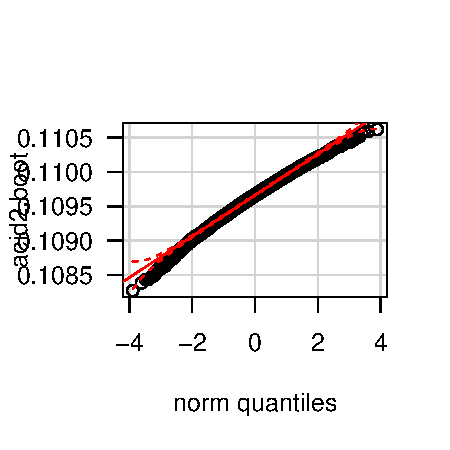
\includegraphics[width=\maxwidth]{figure/2_acid2_qqbott} 

\end{knitrout}
\end{center}\caption{QQ Plot of Acid 2 Concentration Bootstrap Sample Distribution.} \end{figure}

\begin{itemize}
\item Acid 2 Bootstrap Sample Distribtion:  The Acid 2 bootstrap sample distribution is unimodal ish, normal, and contains outliers.  The mean of the data is inside of the IQR and the tails are nearly equal length. The QQ plot of the data shows the are normally distributed, as they follow the line representing normality very closely.
\end{itemize}

\subsection{(20 pts)Formally compare the experiments using two-sample t-procedures.}

\begin{itemize}
  \item Definition of Population Parameters: $\mu = \mu_1 - \mu_2 = $  The population parameter is  the difference in the population mean acid concentration between Acid 1 and Acid 2.
  \item Hypothesis:  Is it plausible that the difference in the population mean acid concentration is different from zero.  In notation:  $H_0: \mu_1 - \mu_2 = 0$ versus $H_A: \mu_1 - \mu_2 \ne 0$

\begin{knitrout}
\definecolor{shadecolor}{rgb}{0.969, 0.969, 0.969}\color{fgcolor}\begin{kframe}
\begin{alltt}
\hlcom{# summary of statistics}
\hlstd{m1} \hlkwb{<-} \hlkwd{mean}\hlstd{(acid1}\hlopt{$}\hlstd{conc)}
\hlstd{s1} \hlkwb{<-} \hlkwd{sd}\hlstd{(acid1}\hlopt{$}\hlstd{conc)}
\hlstd{n1} \hlkwb{<-} \hlkwd{length}\hlstd{(acid1}\hlopt{$}\hlstd{conc)}
\hlstd{m2} \hlkwb{<-} \hlkwd{mean}\hlstd{(acid2}\hlopt{$}\hlstd{conc)}
\hlstd{s2} \hlkwb{<-} \hlkwd{sd}\hlstd{(acid2}\hlopt{$}\hlstd{conc)}
\hlstd{n2} \hlkwb{<-} \hlkwd{length}\hlstd{(acid2}\hlopt{$}\hlstd{conc)}

\hlkwd{c}\hlstd{(m1, s1, n1)} \hlcom{#Acid 1 statistics}
\end{alltt}
\begin{verbatim}
## [1] 1.101e-01 4.544e-03 1.240e+02
\end{verbatim}
\begin{alltt}
\hlkwd{c}\hlstd{(m2, s2, n2)} \hlcom{#Acid 2 Statistics}
\end{alltt}
\begin{verbatim}
## [1]  0.109649  0.001844 37.000000
\end{verbatim}
\begin{alltt}
\hlcom{# Two sample T Test test with pooled variance}
\hlstd{d2.t} \hlkwb{<-} \hlkwd{t.test}\hlstd{(acid1}\hlopt{$}\hlstd{conc, acid2}\hlopt{$}\hlstd{conc,} \hlkwc{var.equal} \hlstd{=} \hlnum{TRUE}\hlstd{)}
\hlstd{d2.t}
\end{alltt}
\begin{verbatim}
## 
## 	Two Sample t-test
## 
## data:  acid1$conc and acid2$conc
## t = 0.5426, df = 159, p-value = 0.5882
## alternative hypothesis: true difference in means is not equal to 0
## 95 percent confidence interval:
##  -0.001098  0.001930
## sample estimates:
## mean of x mean of y 
##    0.1101    0.1096
\end{verbatim}
\end{kframe}
\end{knitrout}

\item  Summary:  The pooled analysis suggests that the difference in the mean precipitation volume is  zero.  The t-statistic was 0.5 and two-sided p-value was 0.6 therefore, because the p-value is greater than 0.05, I fail to reject the Null hypothesis ($H_0: \mu_1 - \mu_2 = 0$) in favor of the Alternative hypothesis ($H_A: \mu_1 - \mu_2 \ne 0$).  The Difference in the population mean acid concentration between Acid 1 and Acid 2 are not different.  \

With 95\% confidence, the difference in the poulation mean acid concentration ($\mu_1 - \mu_2$) is between $-1.1 \times 10 ^{-3}$ and $2.0 \times 10^{-3}$  That is, I am $95\%$ confident that the population mean acid concentration for Acid 1 $\mu_1$ does not exceed the population mean acid concentration for Acid 2 $\mu_2$.

\end{itemize}

\begin{figure}[H]  \begin{center}
\begin{knitrout}
\definecolor{shadecolor}{rgb}{0.969, 0.969, 0.969}\color{fgcolor}\begin{kframe}
\begin{alltt}
\hlcom{#### Visual comparison of whether sampling distribution is close to Normal via Bootstrap}
\hlstd{acid1.num} \hlkwb{<-} \hlstd{acid1[,}\hlnum{1}\hlstd{]}
\hlstd{acid2.num} \hlkwb{<-} \hlstd{acid2[,}\hlnum{1}\hlstd{]}
\hlkwd{bs.two.samp.diff.dist}\hlstd{(acid1.num, acid2.num)}
\end{alltt}
\end{kframe}
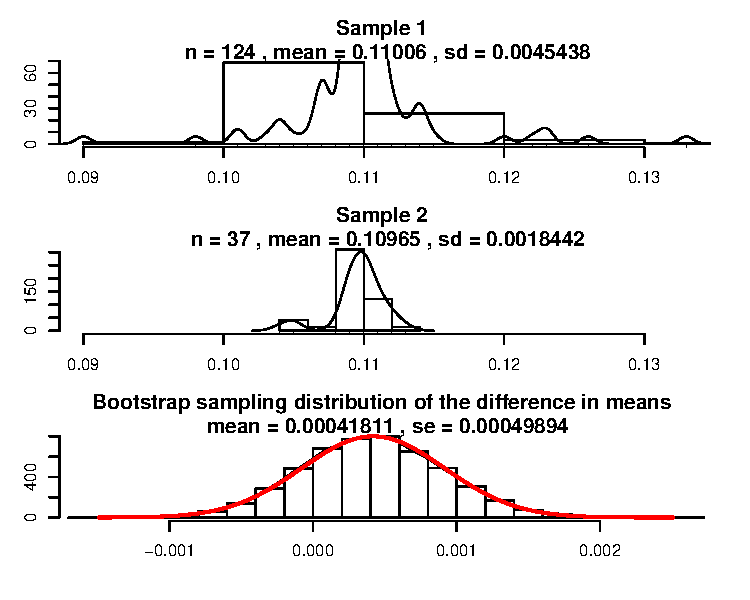
\includegraphics[width=\maxwidth]{figure/2b_bootstrap} 

\end{knitrout}
\end{center} \caption{Bootstrap Sampling Distribution of Pooled Acid Data.} \end{figure}

\begin{itemize}
\item Assumptions:  The pooled variance method assumes the populations have normal frequency curves, with similar population standard deviations.  As shown above, the distribution of difference in means is very close to normal.
\end{itemize}

%%%%%%%%%%%%%%%%%%%%%%%%%
%%%%%%%%%%%%%%%%%%%%%%%%%
%%% Problem 3
%%%%%%%%%%%%%%%%%%%%%%%%%
%%%%%%%%%%%%%%%%%%%%%%%%%
\section{cAMP}
\begin{knitrout}
\definecolor{shadecolor}{rgb}{0.969, 0.969, 0.969}\color{fgcolor}\begin{kframe}
\begin{alltt}
\hlstd{d3} \hlkwb{<-} \hlkwd{read.csv}\hlstd{(}\hlstr{"http://statacumen.com/teach/ADA1/ADA1_HW_03_F14-3.csv"}\hlstd{)}
\hlstd{Dif} \hlkwb{<-} \hlstd{d3}\hlopt{$}\hlstd{Control} \hlopt{-} \hlstd{d3}\hlopt{$}\hlstd{Progesterone}
\hlstd{frog} \hlkwb{<-} \hlkwd{data.frame}\hlstd{(}\hlkwd{cbind}\hlstd{(d3,Dif))}
\end{alltt}
\end{kframe}
\end{knitrout}

The population parameter is the average difference between the cAMP levels for the control and progesterone samples.

\subsection{(10 pts) Make a histogram and box plot of the differences between the cAMP levels for the control and progesterone samples.}

\begin{knitrout}
\definecolor{shadecolor}{rgb}{0.969, 0.969, 0.969}\color{fgcolor}\begin{kframe}
\begin{alltt}
\hlcom{# histogram of frog}
\hlstd{frog.hist} \hlkwb{<-} \hlkwd{ggplot}\hlstd{(frog,} \hlkwd{aes}\hlstd{(}\hlkwc{x} \hlstd{= Dif))}
\hlstd{frog.hist} \hlkwb{<-} \hlstd{frog.hist} \hlopt{+} \hlkwd{geom_histogram}\hlstd{(}\hlkwc{binwidth} \hlstd{=} \hlnum{.1}\hlstd{)}

\hlcom{# boxplot of frog}
\hlstd{frog.box} \hlkwb{<-} \hlkwd{ggplot}\hlstd{(frog,} \hlkwd{aes}\hlstd{(}\hlkwc{x} \hlstd{=} \hlstr{"Difference in cAMP"}\hlstd{,} \hlkwc{y} \hlstd{= Dif))} \hlcom{# boxplot of frog}
\hlstd{frog.box} \hlkwb{<-} \hlstd{frog.box} \hlopt{+} \hlkwd{geom_boxplot}\hlstd{()}
\hlstd{frog.box} \hlkwb{<-} \hlstd{frog.box} \hlopt{+} \hlkwd{coord_flip}\hlstd{()}
\hlstd{frog.box} \hlkwb{<-} \hlstd{frog.box} \hlopt{+} \hlkwd{stat_summary}\hlstd{(}\hlkwc{fun.y} \hlstd{= mean,} \hlkwc{geom} \hlstd{=} \hlstr{"point"}\hlstd{,} \hlkwc{shape} \hlstd{=} \hlnum{3}\hlstd{,} \hlkwc{size} \hlstd{=} \hlnum{2}\hlstd{)}
\end{alltt}
\end{kframe}
\end{knitrout}

\begin{figure}[H]  \begin{center}
\begin{knitrout}
\definecolor{shadecolor}{rgb}{0.969, 0.969, 0.969}\color{fgcolor}\begin{kframe}
\begin{alltt}
\hlcom{# plot histogram and boxplot}
\hlkwd{grid.arrange}\hlstd{(frog.hist, frog.box,} \hlkwc{nrow} \hlstd{=} \hlnum{2}\hlstd{)}
\end{alltt}
\end{kframe}
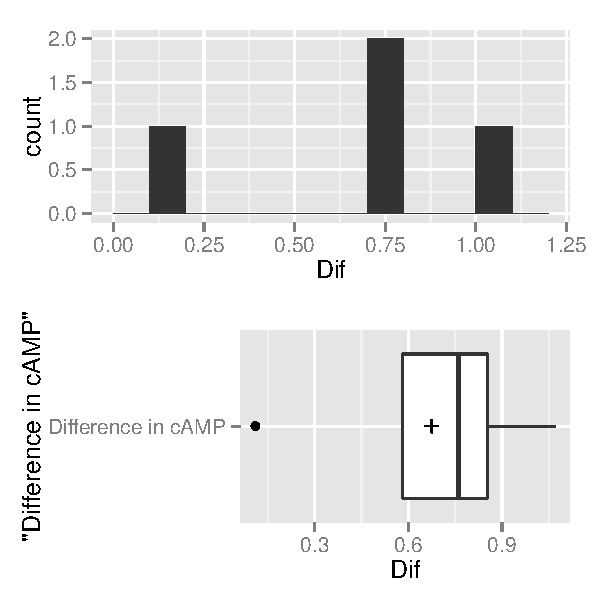
\includegraphics[width=\maxwidth]{figure/2_frog_boxplot} 

\end{knitrout}
\end{center} \caption{Histogram and Boxplot of Difference.} \end{figure}

\begin{itemize}
\item Differences Between the cAMP Levels:  The distribution is uniform, contains outliers, and is skewed right.  The mean of the data is inside of the IQR.
\end{itemize}

\subsection{(20 pts) Test at the 10\% level whether there is any difference in the population mean cAMP levels for batches of oocytes that are untreated versus those treated with progesterone.}


\begin{figure}[H]  \begin{center}
\begin{knitrout}
\definecolor{shadecolor}{rgb}{0.969, 0.969, 0.969}\color{fgcolor}\begin{kframe}
\begin{alltt}
\hlstd{frog.boot} \hlkwb{<-} \hlkwd{bs.one.samp.dist}\hlstd{(frog}\hlopt{$}\hlstd{Dif)}      \hlcom{# plot histogram and frequency density curve}
\end{alltt}
\end{kframe}
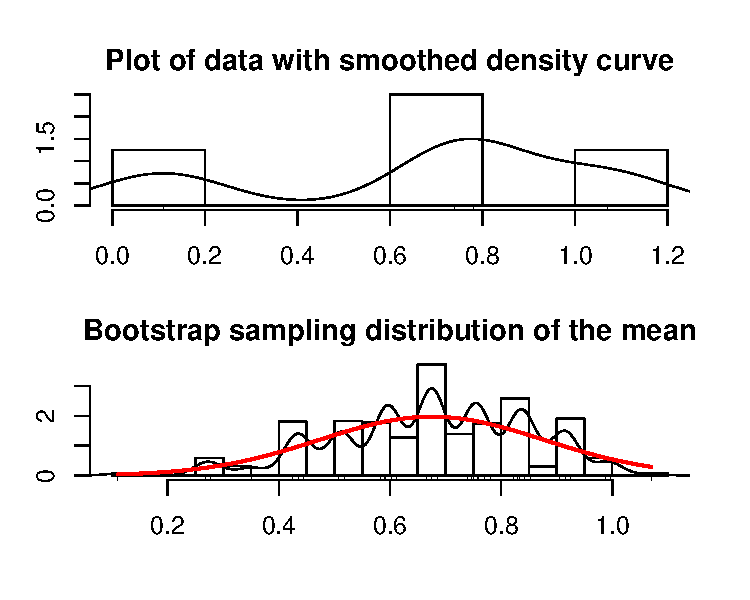
\includegraphics[width=\maxwidth]{figure/2_frog_boot} 

\end{knitrout}
\end{center}\caption{Bootstrap Sample Distribution of the cAMP difference.} \end{figure}

\begin{knitrout}
\definecolor{shadecolor}{rgb}{0.969, 0.969, 0.969}\color{fgcolor}\begin{kframe}
\begin{alltt}
\hlstd{frog.boot.df} \hlkwb{<-} \hlkwd{data.frame}\hlstd{((frog.boot))}

\hlcom{# histogram of frog}
\hlstd{frog.hist.boot} \hlkwb{<-} \hlkwd{ggplot}\hlstd{(frog.boot.df,} \hlkwd{aes}\hlstd{(}\hlkwc{x} \hlstd{= X.frog.boot.))}
\hlstd{frog.hist.boot} \hlkwb{<-} \hlstd{frog.hist.boot} \hlopt{+} \hlkwd{geom_histogram}\hlstd{(}\hlkwc{binwidth} \hlstd{=} \hlnum{.05}\hlstd{)}

\hlcom{# boxplot of frog}
\hlstd{frog.box.boot} \hlkwb{<-} \hlkwd{ggplot}\hlstd{(frog.boot.df,} \hlkwd{aes}\hlstd{(}\hlkwc{x} \hlstd{=} \hlstr{"Concentration"}\hlstd{,} \hlkwc{y} \hlstd{= X.frog.boot.))} \hlcom{# boxplot of frog}
\hlstd{frog.box.boot} \hlkwb{<-} \hlstd{frog.box.boot} \hlopt{+} \hlkwd{geom_boxplot}\hlstd{()}
\hlstd{frog.box.boot} \hlkwb{<-} \hlstd{frog.box.boot} \hlopt{+} \hlkwd{coord_flip}\hlstd{()}
\hlstd{frog.box.boot} \hlkwb{<-} \hlstd{frog.box.boot} \hlopt{+} \hlkwd{stat_summary}\hlstd{(}\hlkwc{fun.y} \hlstd{= mean,} \hlkwc{geom} \hlstd{=} \hlstr{"point"}\hlstd{,} \hlkwc{shape} \hlstd{=} \hlnum{3}\hlstd{,} \hlkwc{size} \hlstd{=} \hlnum{2}\hlstd{)}
\end{alltt}
\end{kframe}
\end{knitrout}

\begin{figure}[H]  \begin{center}
\begin{knitrout}
\definecolor{shadecolor}{rgb}{0.969, 0.969, 0.969}\color{fgcolor}\begin{kframe}
\begin{alltt}
\hlcom{# plot histogram and boxplot}
\hlkwd{grid.arrange}\hlstd{(frog.hist.boot, frog.box.boot,} \hlkwc{nrow} \hlstd{=} \hlnum{2}\hlstd{)}
\end{alltt}
\end{kframe}
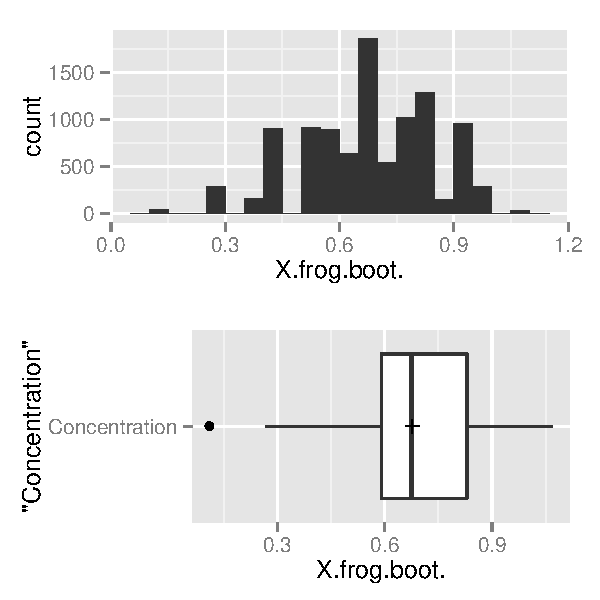
\includegraphics[width=\maxwidth]{figure/2_frog_bootbox_plot} 

\end{knitrout}
\end{center} \caption{Histogram and Boxplot of cAMP Difference Bootstrap Sample Distribution.} \end{figure}

\begin{figure}[H]  \begin{center}
\begin{knitrout}
\definecolor{shadecolor}{rgb}{0.969, 0.969, 0.969}\color{fgcolor}\begin{kframe}
\begin{alltt}
\hlcom{# qq plot for acid 1 concentration data}
\hlkwd{qqPlot}\hlstd{(frog.boot,} \hlkwc{las} \hlstd{=} \hlnum{1}\hlstd{,} \hlkwc{id.n} \hlstd{=} \hlnum{0}\hlstd{,} \hlkwc{id.cex} \hlstd{=} \hlnum{1}\hlstd{,} \hlkwc{lwd} \hlstd{=} \hlnum{1}\hlstd{)}
\end{alltt}
\end{kframe}
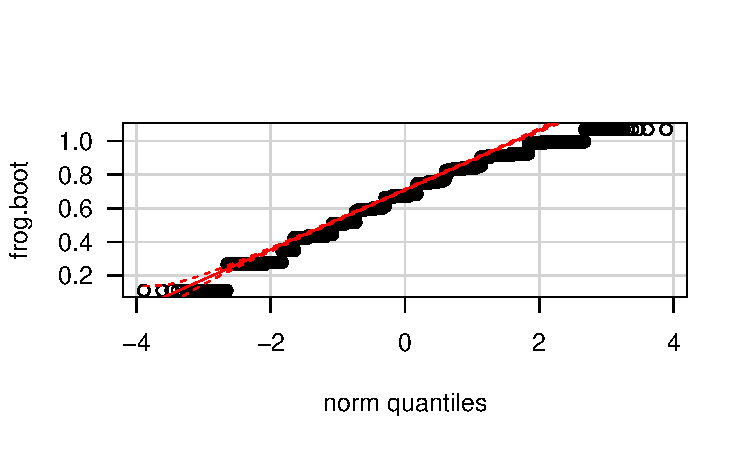
\includegraphics[width=\maxwidth]{figure/2_frog_qqbott} 

\end{knitrout}
\end{center}\caption{QQ Plot of cAMP Difference Bootstrap Sample Distribution.} \end{figure}

\begin{itemize}
\item cAMP Bootstrap Sample Distribtion:  The bootstrap sample distribution is unimodal, not normal, and contains outliers.  The mean of the data is inside of the IQR and the left tail is longer than the right. The QQ plot of the data shows the are not normally distributed.  Because the sample differences are not from a normal population, a one sample technique should not be used.

  \item Definition of Population Parameters: $\mu = \mu_1 - \mu_2 = $  The population parameter is  the difference in the population mean cAMP levels between the oocytes not exposed to progesterone (control) and oocytes exposed to progesterone.
  \item Hypothesis:  Is it plausible that the difference in the population mean cAMP Level is different from zero.  In notation:  $H_0: \mu_1 - \mu_2 = 0$ versus $H_A: \mu_1 - \mu_2 \ne 0$
  \item Results:  The paired analysis suggests that the difference in the mean precipitation volume is  zero.  The t-statistic was 3.3 and two-sided p-value was 0.04 therefore, because the p-value is less than 0.1, I reject the Null hypothesis ($H_0: \mu_1 - \mu_2 = 0$) in favor of the Alternative hypothesis ($H_A: \mu_1 - \mu_2 \ne 0$).  The Difference in the population mean cAMP level between untreated oocytes (control) and those treated with progesterone are different.
  \end{itemize}

\begin{knitrout}
\definecolor{shadecolor}{rgb}{0.969, 0.969, 0.969}\color{fgcolor}\begin{kframe}
\begin{alltt}
\hlcom{# summary of statistics}
\hlstd{m1} \hlkwb{<-} \hlkwd{mean}\hlstd{(frog}\hlopt{$}\hlstd{Control)}
\hlstd{s1} \hlkwb{<-} \hlkwd{sd}\hlstd{(frog}\hlopt{$}\hlstd{Control)}
\hlstd{n1} \hlkwb{<-} \hlkwd{length}\hlstd{(frog}\hlopt{$}\hlstd{Control)}
\hlstd{m2} \hlkwb{<-} \hlkwd{mean}\hlstd{(frog}\hlopt{$}\hlstd{Progesterone)}
\hlstd{s2} \hlkwb{<-} \hlkwd{sd}\hlstd{(frog}\hlopt{$}\hlstd{Progesterone)}
\hlstd{n2} \hlkwb{<-} \hlkwd{length}\hlstd{(frog}\hlopt{$}\hlstd{Progesterone)}

\hlkwd{c}\hlstd{(m1, s1, n1)} \hlcom{#Control}
\end{alltt}
\begin{verbatim}
## [1] 2.980 2.047 4.000
\end{verbatim}
\begin{alltt}
\hlkwd{c}\hlstd{(m2, s2, n2)} \hlcom{#Progesterone}
\end{alltt}
\begin{verbatim}
## [1] 2.305 1.952 4.000
\end{verbatim}
\begin{alltt}
\hlcom{# Paired Two sample T Test with CI at 90%}
\hlstd{frog.t} \hlkwb{<-} \hlkwd{t.test}\hlstd{(frog}\hlopt{$}\hlstd{Control, frog}\hlopt{$}\hlstd{Progesterone,} \hlkwc{paired} \hlstd{=} \hlnum{TRUE}\hlstd{,} \hlkwc{conf.level} \hlstd{=} \hlnum{0.9}\hlstd{)}
\hlstd{frog.t}
\end{alltt}
\begin{verbatim}
## 
## 	Paired t-test
## 
## data:  frog$Control and frog$Progesterone
## t = 3.339, df = 3, p-value = 0.04443
## alternative hypothesis: true difference in means is not equal to 0
## 90 percent confidence interval:
##  0.1992 1.1508
## sample estimates:
## mean of the differences 
##                   0.675
\end{verbatim}
\end{kframe}
\end{knitrout}



\subsection{(10 pts) Compute and interpret a 90\% CI for the difference in population mean cAMP levels for batches of oocytes that are untreated versus those treated with progesterone.}

With 90\% confidence, the difference in the poulation mean cAMP level ($\mu_1 - \mu_2$) is between 0.2  and 1.2.  That is, I am $90\%$ confident that the population mean cAMP level for untreated oocytes (control) $\mu_1$ exceeds the population mean cAMP level for treated oocytes $\mu_2$ by between 0.2 and 1.2 pmol/oocyte.

\subsection{(10 pts) Discuss any statistical assumptions that you have made in carrying out the analysis, and whether the assumptions seem reasonable.}

The paired variance method assumes the paired differences have normal frequency curves, with similar population standard deviations.  As shown above, the distribution of difference in means is not normal.  We also assume the data were randomly sampled.

\subsection{(10 pts) Write a short summary to the problem.}

The paired analysis suggests that the difference in the mean precipitation volume is  zero.  The t-statistic was 3.3 and two-sided p-value was 0.04 therefore, because the p-value is less than 0.1, I reject the Null hypothesis ($H_0: \mu_1 - \mu_2 = 0$) in favor of the Alternative hypothesis ($H_A: \mu_1 - \mu_2 \ne 0$).  The Difference in the population mean cAMP level between untreated oocytes (control) and those treated with progesterone are different.  That is, I am $90\%$ confident that the population mean cAMP level for untreated oocytes (control) $\mu_1$ exceeds the population mean cAMP level for treated oocytes $\mu_2$ by between 0.2 and 1.2 pmol/oocyte.

\end{document}
